\documentclass[11pt,a4paper]{article}

\usepackage[utf8]{inputenc}
\usepackage[T1]{fontenc}
\usepackage[spanish,es-nodecimaldot]{babel}
\usepackage{amsmath}
\usepackage{booktabs}
\usepackage{tabularx}
\usepackage{array}
\usepackage{graphicx}
\usepackage{geometry}
\usepackage{xcolor}
\usepackage{float}
\usepackage{caption}
\usepackage[numbers,sort&compress]{natbib}
\usepackage{hyperref}
\geometry{margin=2.2cm}
\hypersetup{
    colorlinks=true,
    linkcolor=blue!50!black,
    urlcolor=blue!50!black,
    pdftitle={Reporte integral de la fase stop-band residual},
    pdfauthor={Cesar Zapata}
}

\newcolumntype{Y}{>{\raggedright\arraybackslash}X}

\title{Reporte integral de la fase stop-band residual\\\large Proyecto TD3 para pr\'otesis mioel\'ectrica}
\author{C\'esar Zapata\\Research Laboratory in Artificial Intelligence and Computer Vision ``Alan Turing''}
\date{5 de abril de 2026}

\begin{document}
\maketitle

\section*{Prop\'osito de este documento}
Este documento ordena la fase stop-band residual siguiendo la misma l\'inea de los reportes previos del proyecto. Primero fija cu\'al era la l\'inea vigente antes de la intervenci\'on, luego explica por qu\'e fue necesario abrir esta fase y finalmente resume qu\'e se aplic\'o y qu\'e resultado dej\'o.

\section*{L\'inea vigente antes de la intervenci\'on stop-band}
La fase stop-band \textbf{no} arranc\'o desde cero. Antes de abrirla, el proyecto ya ten\'ia una l\'inea t\'ecnica bien definida:
\begin{itemize}
\item \textbf{benchmark oficial estable:} \texttt{Agent7250};
\item \textbf{mejor residual reproducible:} \texttt{seed 22}, aceptada bajo \texttt{ConditionA};
\item \textbf{mejor residual single-run hist\'orico:} \texttt{Agent1850}, aceptado bajo \texttt{ConditionB}.
\end{itemize}

Ese estado se consolid\'o en la propia secuencia de reportes del proyecto: primero se cerr\'o una base estable sobre \texttt{Agent7250}, despu\'es se abri\'o la l\'inea residual y finalmente se verific\'o qu\'e parte de esa mejora se sosten\'ia entre seeds. Por eso la fase stop-band parte de una l\'inea ya madura: no entra a resolver tracking desde cero, sino a decidir d\'onde conviene detener una trayectoria residual que ya mostraba se\~nales buenas, pero todav\'ia no estaba bien cerrada como regla operativa. Esta lectura es consistente con el uso de TD3 como base de control continuo y con la idea de aprendizaje residual sobre una pol\'itica ya fuerte, especialmente en tareas donde no basta con seguir la referencia, sino que tambi\'en importa la agresividad del control y la calidad operativa de la acci\'on \citep{fujimoto2018td3,silver2018residual,chen2023review,done2025prostheticrl}.

\begin{table}[H]
\centering
\caption{Referencias activas del proyecto antes de stop-band}
\begin{tabularx}{\linewidth}{>{\raggedright\arraybackslash}p{2.6cm} >{\raggedright\arraybackslash}p{2.2cm} Y}
\toprule
Rol & Candidato & Lectura t\'ecnica \\
\midrule
Benchmark oficial & \texttt{Agent7250} & Pol\'itica base estable del proyecto; punto fijo para todas las comparaciones posteriores. \\
Residual reproducible & \texttt{seed 22} & Mejor evidencia entre seeds; referencia operativa de reproducibilidad antes de stop-band. \\
Residual single-run & \texttt{Agent1850} & Mejor compromiso hist\'orico esfuerzo--saturaci\'on en una sola corrida; muy fuerte como referencia cualitativa, pero no suficiente por s\'i solo como l\'inea reproducible. \\
\bottomrule
\end{tabularx}
\end{table}

\begin{figure}[H]
\centering
\begin{minipage}[t]{0.49\linewidth}
\centering
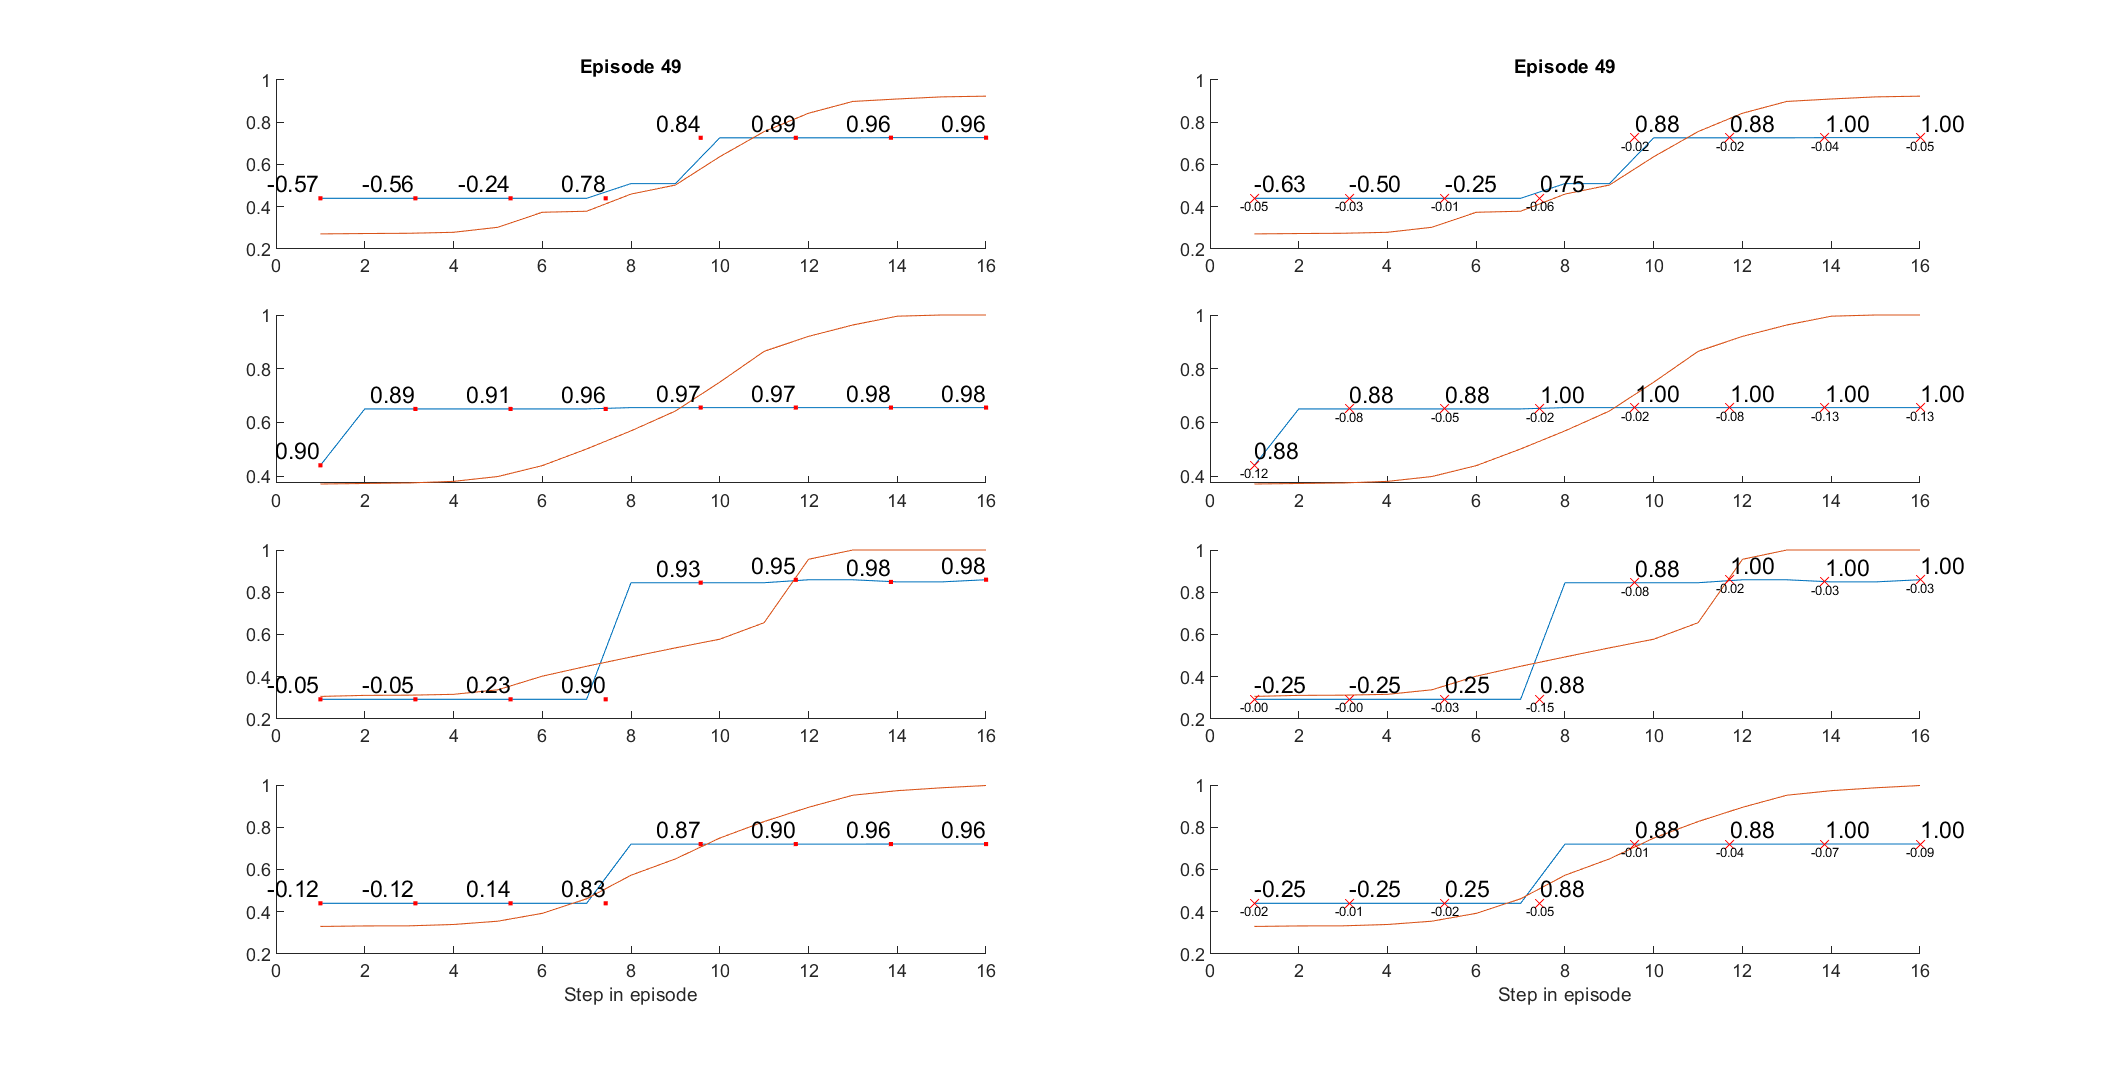
\includegraphics[width=\linewidth]{figures/test_episode_49_valid_baseline_8000.png}
\caption*{(a) \texttt{Agent7250}}
\end{minipage}\hfill
\begin{minipage}[t]{0.49\linewidth}
\centering
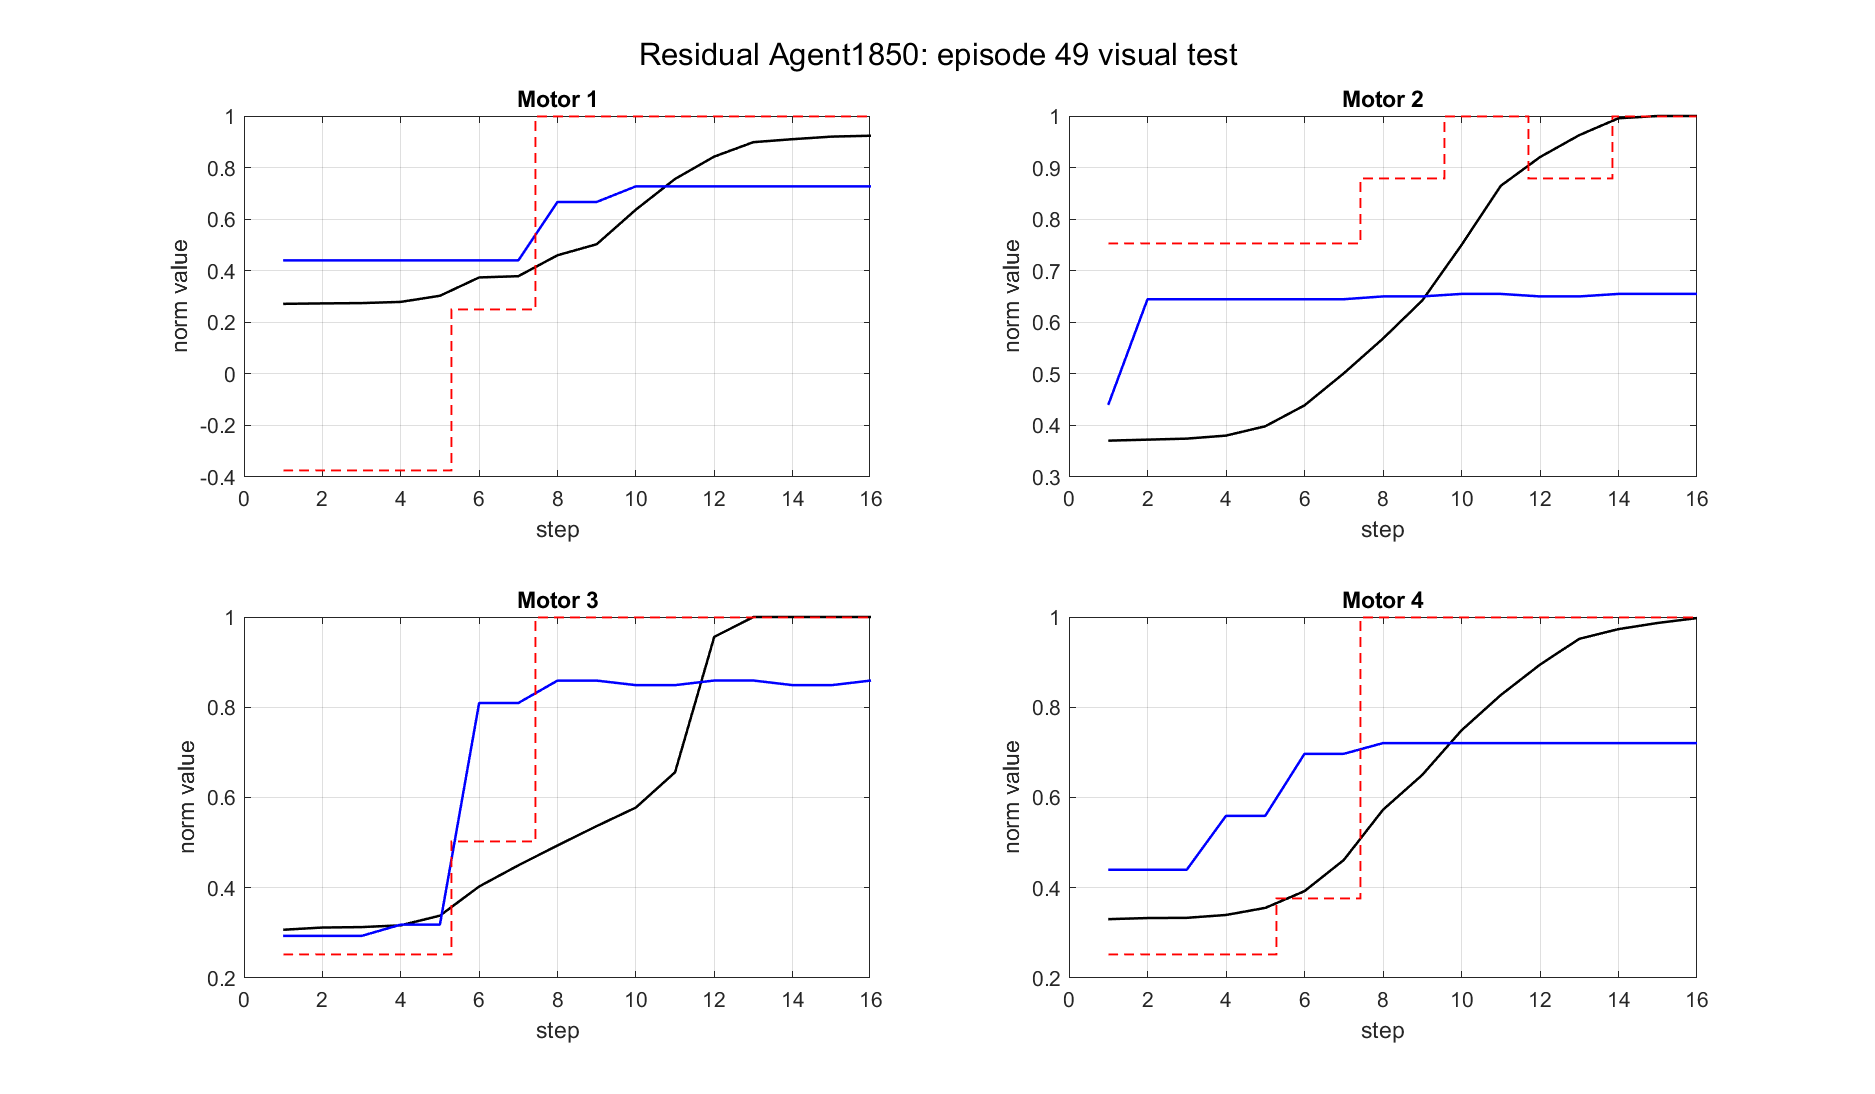
\includegraphics[width=\linewidth]{figures/residual_agent1850_episode49_20260326.png}
\caption*{(b) \texttt{Agent1850}}
\end{minipage}
\caption{L\'inea vigente antes de stop-band. A la izquierda, el benchmark oficial ya resolv\'ia bien el tracking. A la derecha, la mejor residual single-run mostraba que s\'i exist\'ia margen para bajar esfuerzo y saturaci\'on sin destruir el seguimiento.}
\label{fig:linea_previa}
\end{figure}

\section*{Por qu\'e fue necesario abrir una fase stop-band}
El siguiente paso natural habr\'ia sido seguir entrenando m\'as tiempo. Sin embargo, esa hip\'otesis ya fue puesta a prueba con dos corridas largas de \(50{,}000\) episodios: una sobre la base y otra sobre la l\'inea residual. El hallazgo fue consistente en ambos casos: aparecieron checkpoints internamente prometedores dentro de la trayectoria, pero el mejor checkpoint auditado no se sostuvo como nuevo l\'ider al repetir el test final independiente.

En otras palabras, las corridas largas cambiaron la pregunta del proyecto. La pregunta dej\'o de ser ``\emph{si entrenar m\'as ayuda}'' y pas\'o a ser ``\emph{en qu\'e zona de la trayectoria conviene detenerse antes de la deriva tard\'ia}''.

\begin{quote}
En este proyecto, \textbf{stop-band} no se refiere a un filtro en frecuencia sobre la se\~nal EMG. Se refiere a una \textbf{banda de parada sobre el eje de entrenamiento}: una ventana de episodios en la que conviene buscar y fijar el checkpoint final antes de que la trayectoria empiece a degradarse.
\end{quote}

La consecuencia pr\'actica fue inmediata: en esta fase el criterio se desplaz\'o deliberadamente desde ``seguir entrenando'' hacia ``auditar toda la trayectoria y seleccionar la ventana operativamente m\'as sana''. La pregunta ya no era si hac\'ia falta empujar m\'as episodios, sino en qu\'e zona concreta de la trayectoria aparec\'ia el mejor compromiso antes de que el residual empezara a degradarse. Esta decisi\'on tambi\'en es coherente con observaciones conocidas de deep RL: el entrenamiento prolongado no necesariamente mejora de forma mon\'otona, y en control rob\'otico la suavidad de acci\'on es parte real de la calidad del comportamiento final \citep{nikishin2022primacy,lee2024smoothness}.

\begin{figure}[H]
\centering
\begin{minipage}[t]{0.49\linewidth}
\centering
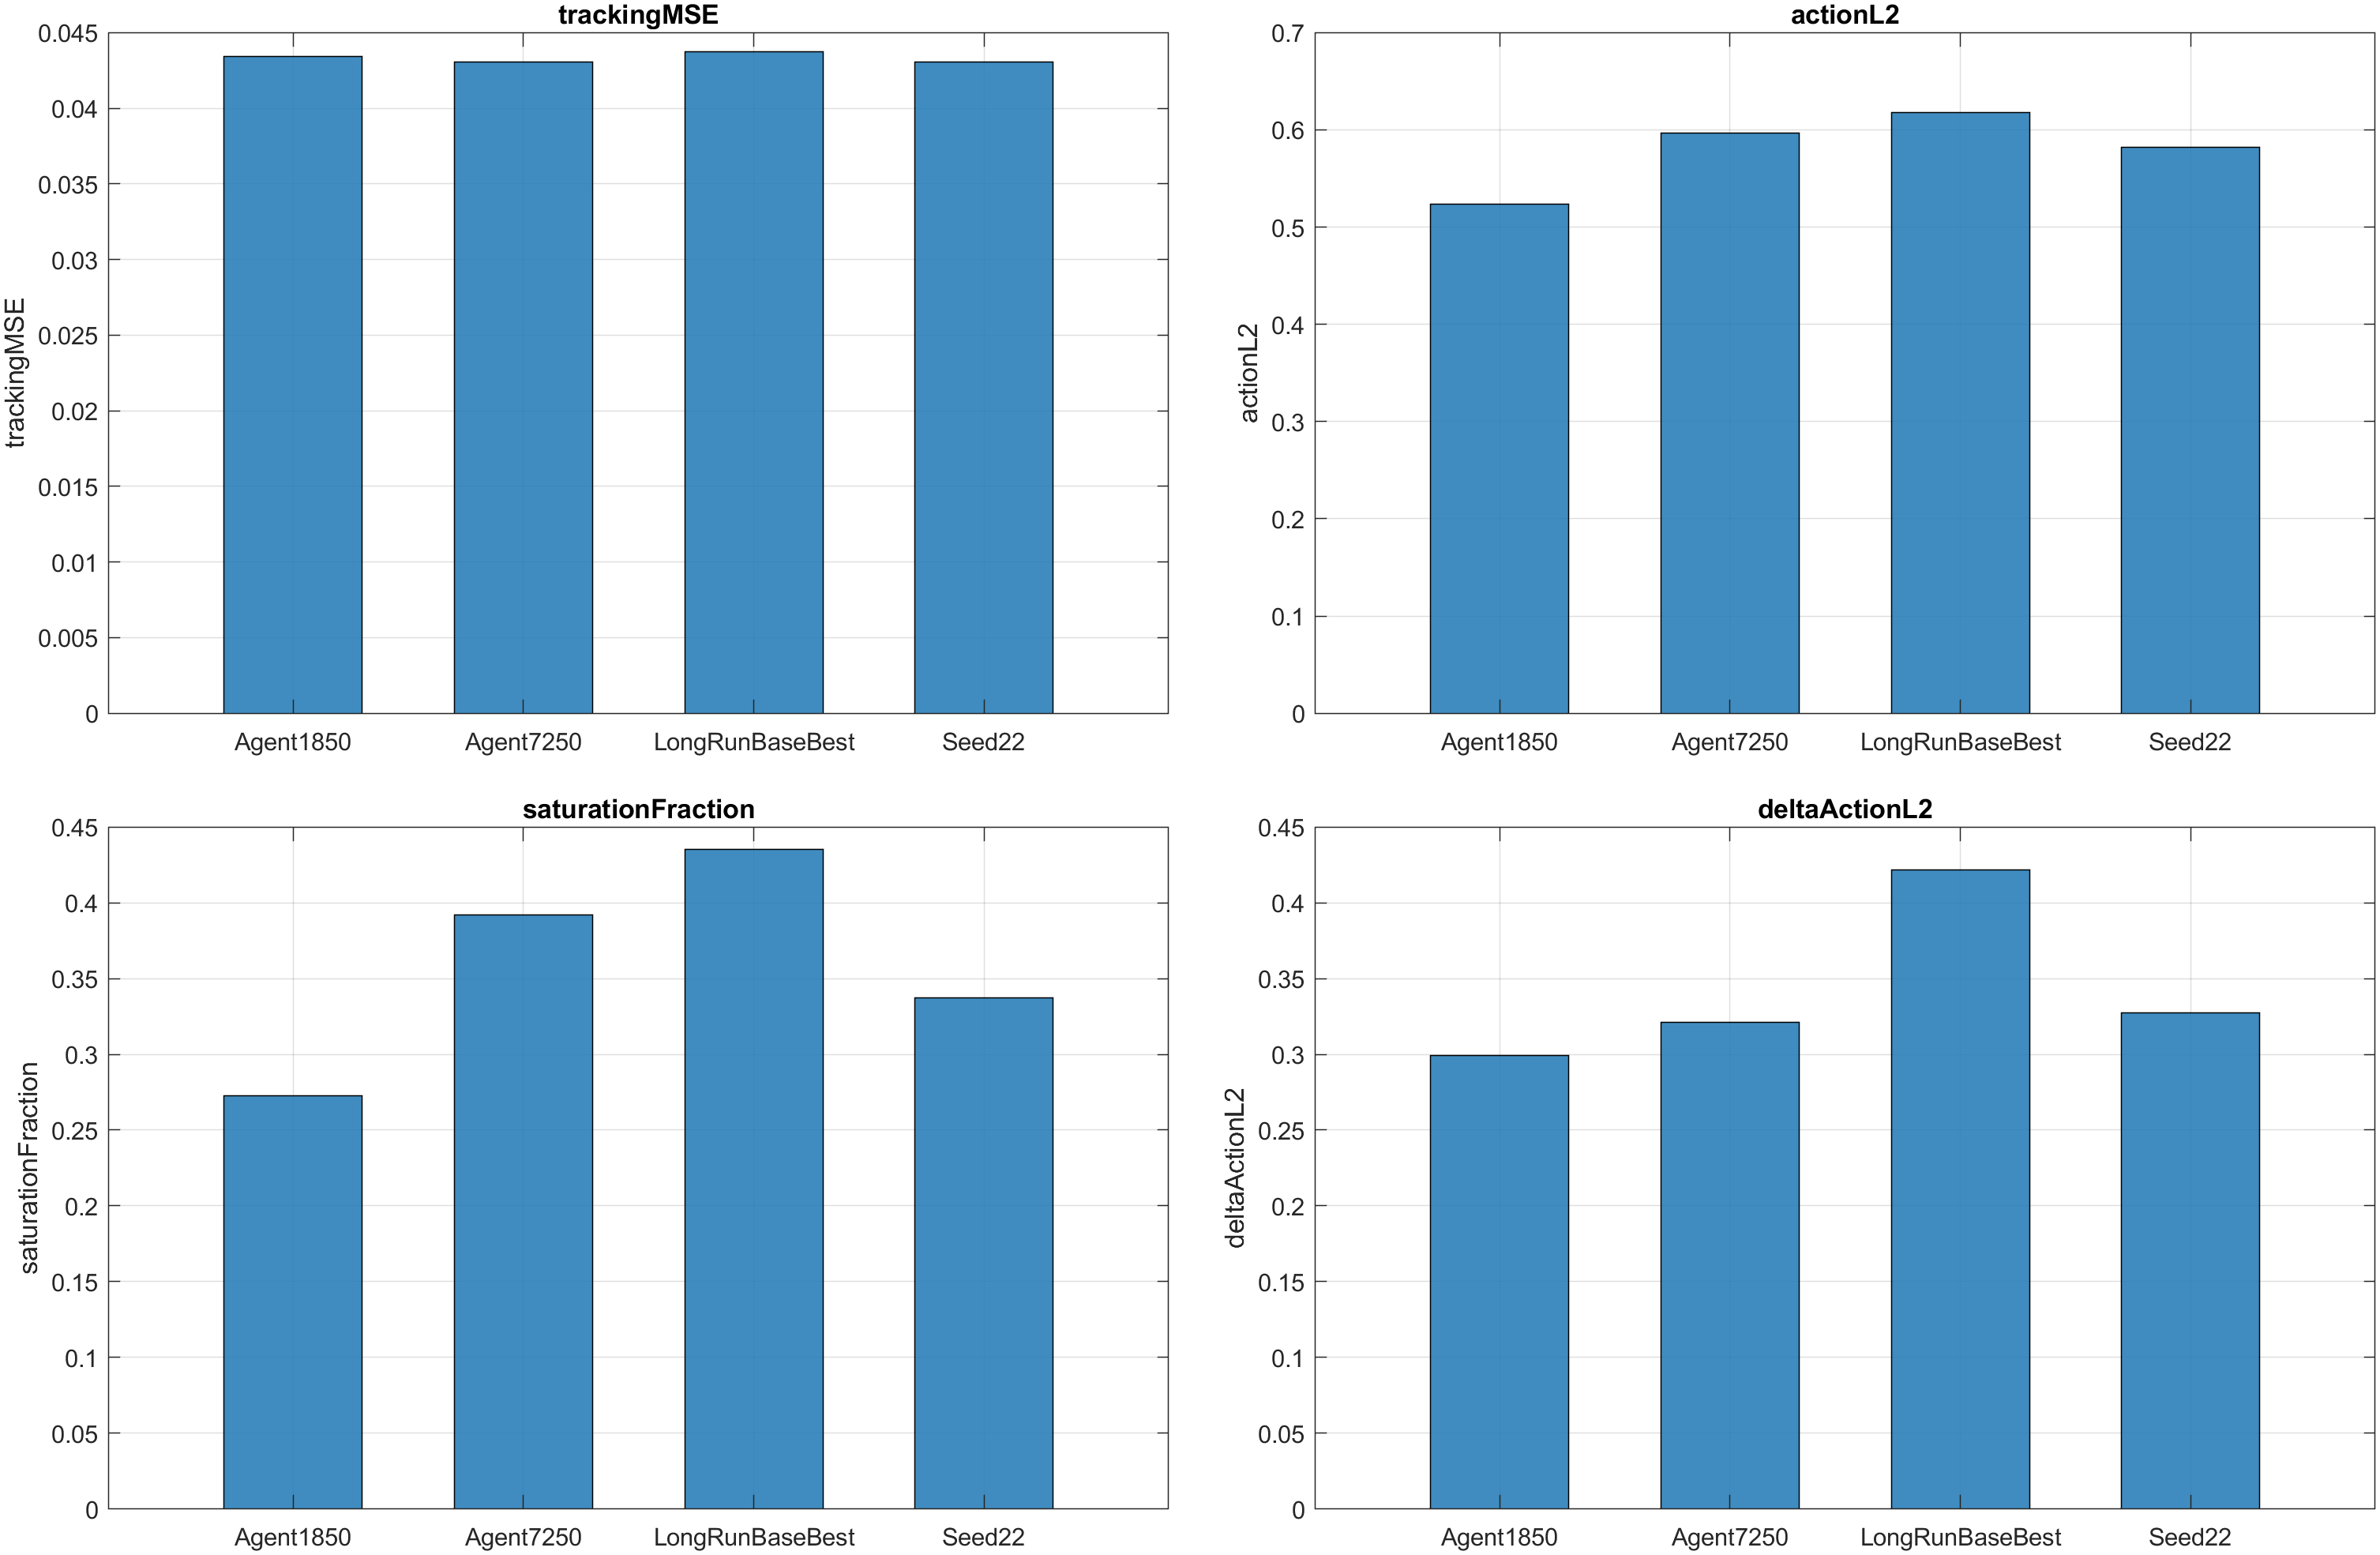
\includegraphics[width=\linewidth]{figures/agent7250_longrun_candidate_comparison_20260404.png}
\caption*{(a) Corrida larga base}
\end{minipage}\hfill
\begin{minipage}[t]{0.49\linewidth}
\centering
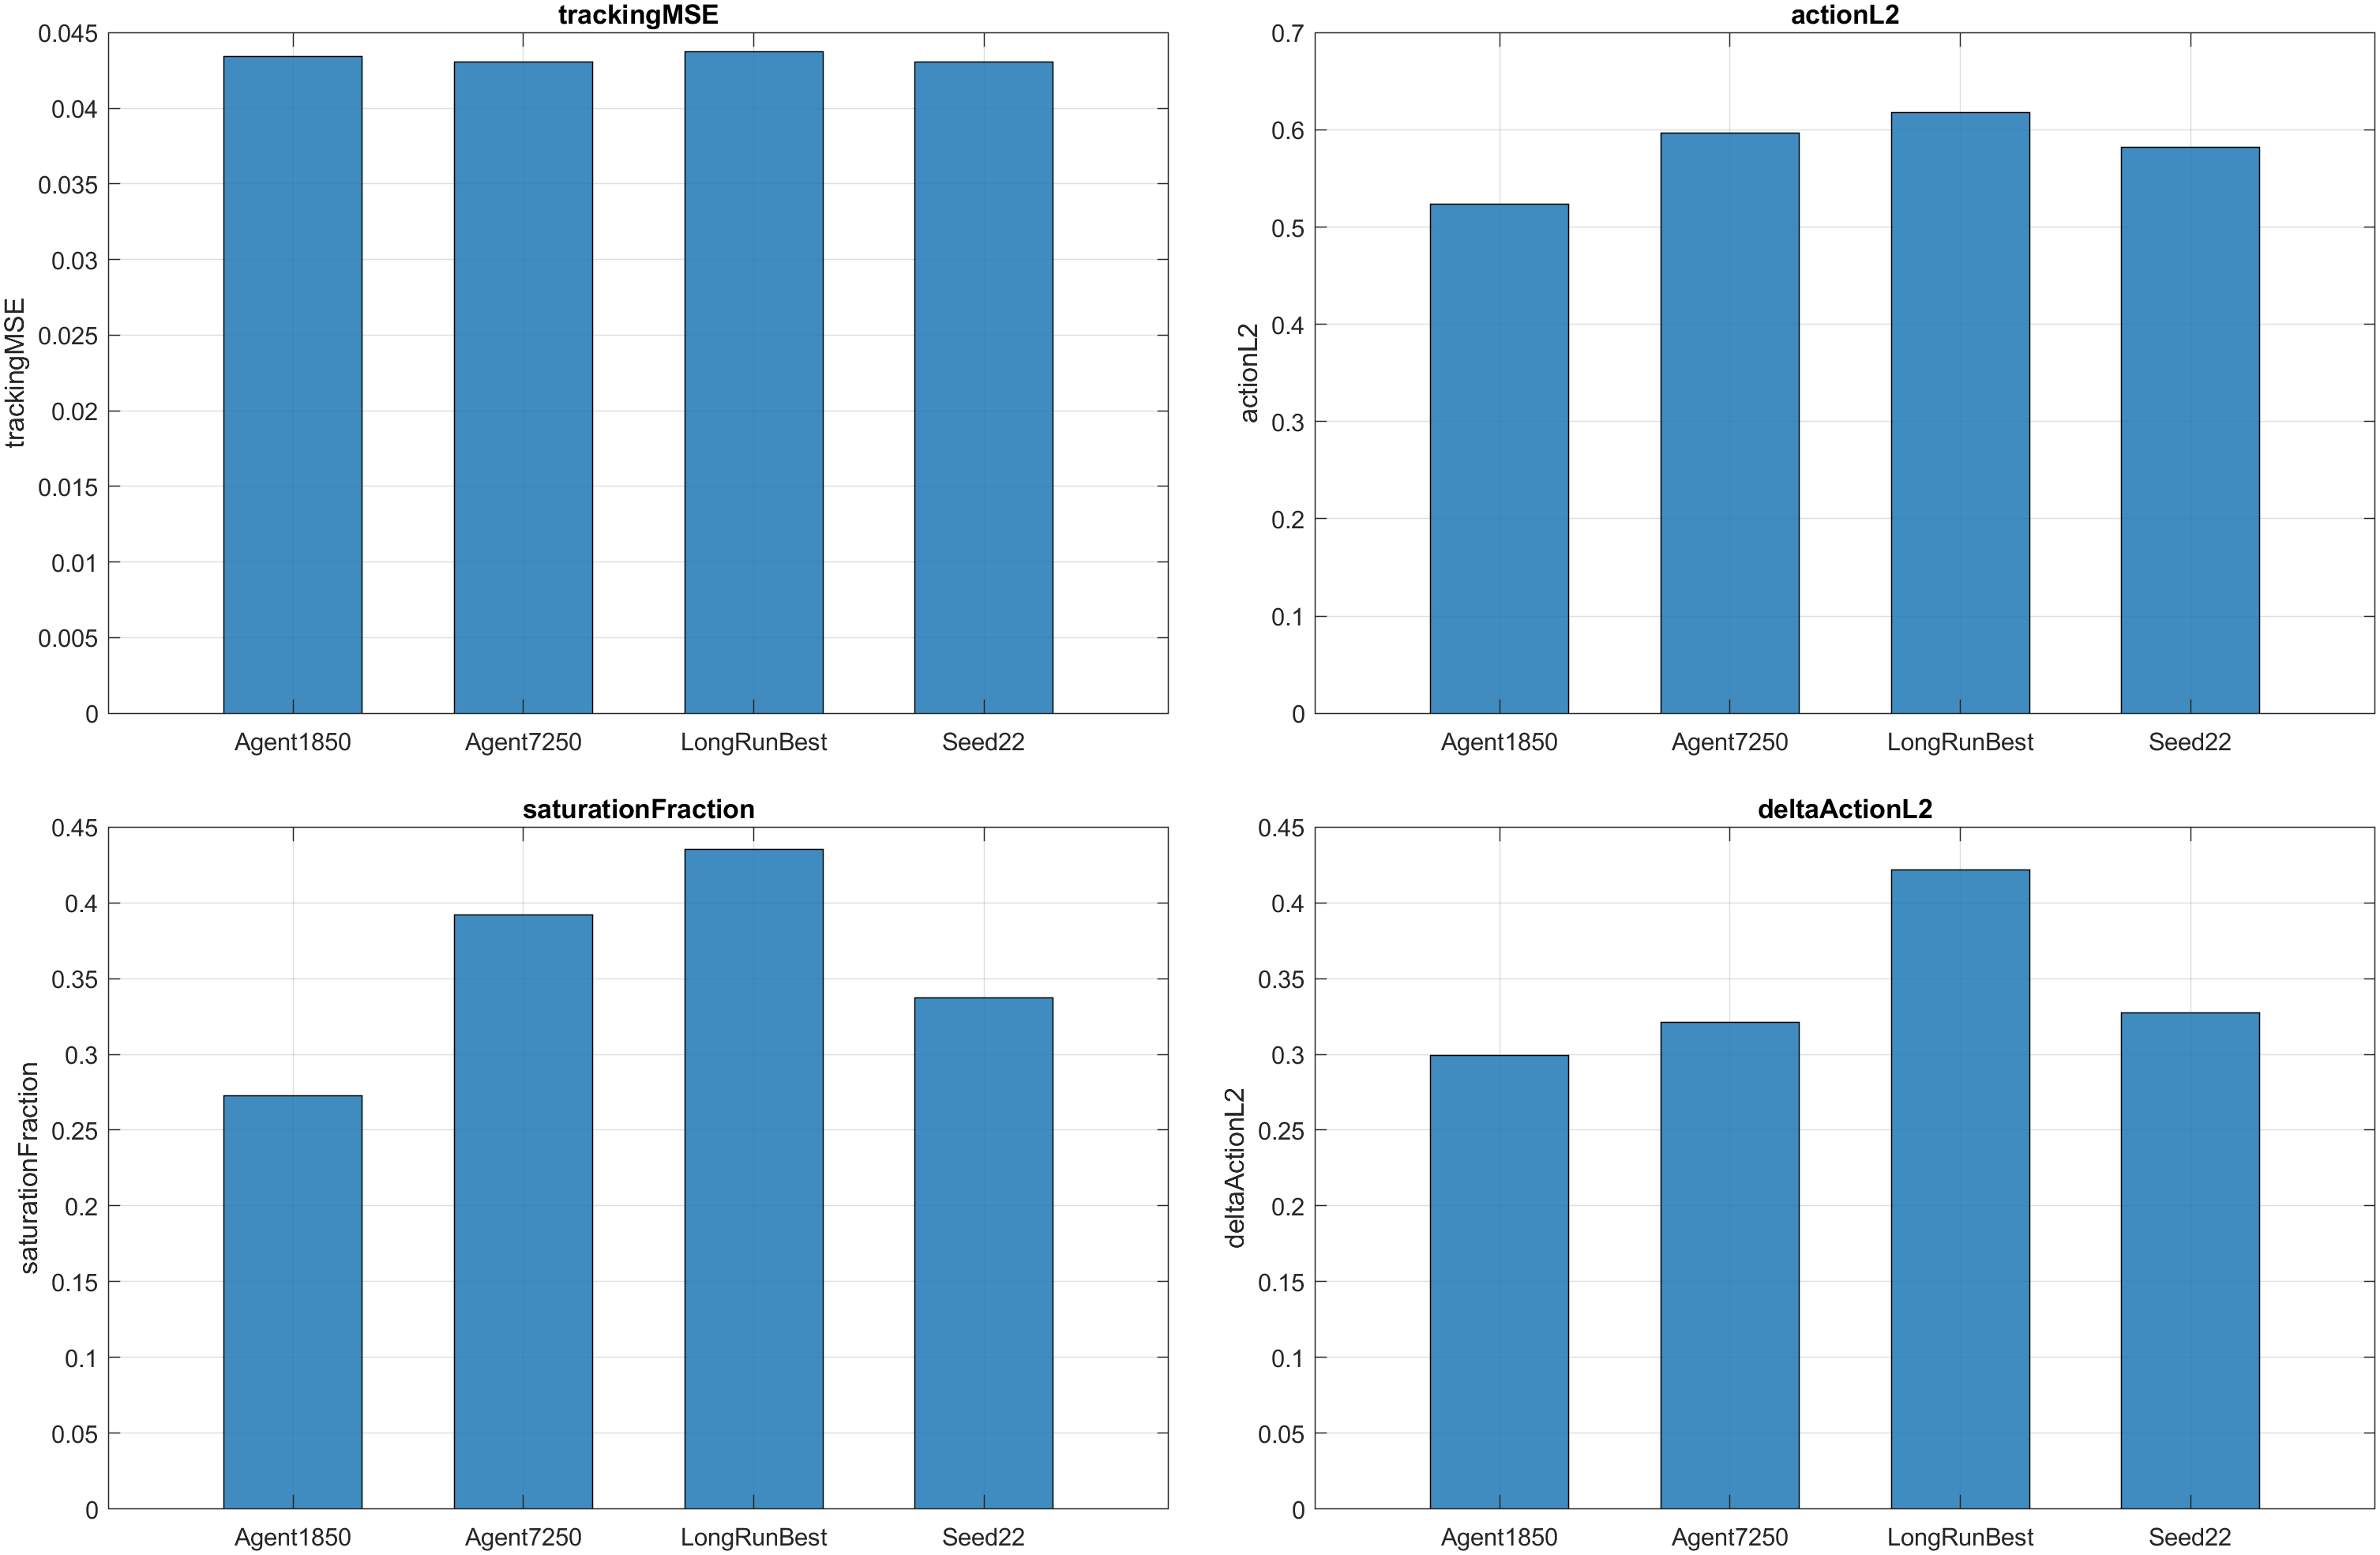
\includegraphics[width=\linewidth]{figures/longrun_residual_candidate_comparison_20260402.png}
\caption*{(b) Corrida larga residual}
\end{minipage}
\caption{Raz\'on inmediata para abrir stop-band. Tanto la extensi\'on larga de la base como la extensi\'on larga residual mostraron que ``m\'as episodios'' no garantizaba un mejor candidato final frente a \texttt{Agent7250}.}
\label{fig:motivacion_longruns}
\end{figure}

\section*{Qu\'e se aplic\'o exactamente}
La intervenci\'on stop-band no cambi\'o el benchmark ni cambi\'o la arquitectura general del proyecto. Lo que hizo fue \textbf{cambiar la forma de buscar y seleccionar el residual}, manteniendo congelada la base \texttt{Agent7250} y volviendo m\'as estricta la auditor\'ia temporal.

\subsection*{1. Pol\'itica residual con base congelada}
La pol\'itica residual activa se mantuvo bajo la forma:
\begin{equation}
a(s) = \mathrm{clip}\Big(a_{\mathrm{base}}(s) + \alpha_{\mathrm{res}}\,a_{\mathrm{res}}(s,a_{\mathrm{base}}), -1, 1\Big),
\label{eq:residual}
\end{equation}
donde \(a_{\mathrm{base}}\) es la acci\'on del benchmark congelado, \(a_{\mathrm{res}}\) es la correcci\'on aprendible y \(\alpha_{\mathrm{res}} = 0.20\) controla cu\'anto puede apartarse la pol\'itica final respecto a la base. En t\'erminos del proyecto, esto significa que la fase stop-band no cambi\'o la l\'ogica residual ya validada; solo cambi\'o la forma de explotar su trayectoria. La estructura mantiene la base TD3 y la correcci\'on residual acotada como elementos centrales del control \citep{fujimoto2018td3,silver2018residual}.

\subsection*{2. Densificaci\'on de checkpoints y auditor\'ia de trayectoria completa}
En vez de confiar en el \'ultimo checkpoint o en el \texttt{AverageReward} final, la fase stop-band aument\'o la densidad de guardado y audit\'o toda la trayectoria:
\begin{itemize}
\item en \emph{discovery}, guardado cada \(250\) episodios;
\item en \emph{confirmation}, guardado cada \(100\) episodios;
\item auditor\'ia en dos fases: \(20\) simulaciones r\'apidas para barrer la trayectoria y \(50\) simulaciones completas para reordenar los mejores candidatos;
\item re-test final independiente del checkpoint seleccionado.
\end{itemize}

\subsection*{3. Regla expl\'icita para derivar la stop-band}
Si \(\mathcal{E}_{\mathrm{acc}}\) es el conjunto de episodios ganadores de las seeds aceptadas, la propuesta de parada se construy\'o como:
\begin{equation}
e^{\star} = \operatorname{round}_{250}\!\left(\operatorname{median}(\mathcal{E}_{\mathrm{acc}})\right),
\label{eq:stopband_median}
\end{equation}
y la ventana asociada como
\begin{equation}
W(e^{\star}) = [e^{\star}-250,\; e^{\star}+250].
\label{eq:stopband_window}
\end{equation}

Cuando \emph{discovery} ten\'ia menos de tres seeds aceptadas, la mediana se mantuvo deliberadamente conservadora y se recort\'o al rango \([1750,3000]\) para no dejar que una sola seed tard\'ia arrastrara toda la fase. Esa fue precisamente la situaci\'on observada en \emph{discovery}.

\subsection*{4. Regla de selecci\'on dentro de la ventana}
En \emph{confirmation} no se eligi\'o simplemente el mejor checkpoint global de la tabla. La regla aplicada fue:
\begin{enumerate}
\item priorizar el \textbf{checkpoint aceptado m\'as temprano} dentro de la ventana \(W(e^{\star})\);
\item si no exist\'ia un aceptado dentro de la ventana, mantener el mejor checkpoint interno de esa banda;
\item solo permitir una promoci\'on fuera de la ventana si mejoraba tracking \textbf{sin} empeorar \texttt{actionL2} ni \texttt{saturationFraction}.
\end{enumerate}

Con esto, la stop-band se convirti\'o en una regla de selecci\'on \emph{conservadora}: la fase prefer\'ia un checkpoint ligeramente m\'as temprano y estable antes que una cola tard\'ia m\'as riesgosa.

\begin{table}[H]
\centering
\caption{Intervenci\'on metodol\'ogica aplicada en la fase stop-band}
\begin{tabularx}{\linewidth}{>{\raggedright\arraybackslash}p{3.3cm} Y}
\toprule
Elemento & Regla aplicada \\
\midrule
Base de partida & \texttt{Agent7250} congelado como benchmark y base residual. \\
Pol\'itica aprendida & Residual TD3 con \(\alpha_{\mathrm{res}} = 0.20\) y \texttt{32} unidades ocultas residuales. \\
Guardado de checkpoints & Denso: cada \(250\) episodios en discovery y cada \(100\) en confirmation. \\
Auditor\'ia & Barrido r\'apido (\(20\) simulaciones), fase completa (\(50\) simulaciones) y re-test final independiente. \\
Derivaci\'on de banda & Mediana de episodios aceptados, redondeada a \(250\), con recorte conservador si la evidencia era escasa. \\
Selecci\'on final & Checkpoint aceptado m\'as temprano dentro de la ventana; solo se sale de la banda si el candidato externo no empeora esfuerzo ni saturaci\'on. \\
Promoci\'on de l\'inea & Requiere simult\'aneamente seeds aceptadas, mejora agregada frente al benchmark y reducci\'on media de \texttt{actionL2} y \texttt{saturationFraction}. \\
\bottomrule
\end{tabularx}
\end{table}

\section*{Discovery: b\'usqueda inicial de la banda}
\subsection*{Configuraci\'on}
\begin{table}[H]
\centering
\caption{Configuraci\'on de discovery}
\begin{tabularx}{\linewidth}{lY}
\toprule
Elemento & Valor \\
\midrule
Base congelada & \texttt{Agent7250} \\
Seeds & \texttt{[11 22 33 44 55]} \\
Episodios por seed & \(10{,}000\) \\
Guardado & cada \(250\) episodios \\
Auditor\'ia & \(20\) simulaciones r\'apidas, \(50\) completas, \(\texttt{topK}=5\) \\
Selecci\'on & auditor\'ia completa + re-test final independiente \\
\bottomrule
\end{tabularx}
\end{table}

\subsection*{Resultado agregado}
\begin{table}[H]
\centering
\caption{Resumen agregado de discovery}
\begin{tabularx}{\linewidth}{l c}
\toprule
M\'etrica & Valor \\
\midrule
Seeds aceptadas & \(1/5\) \\
ConditionA & \(1\) \\
ConditionB & \(0\) \\
Rejected & \(4\) \\
trackingMSE medio \(\pm\) std & \(0.042706 \pm 0.000190\) \\
trackingMAE medio \(\pm\) std & \(0.160010 \pm 0.000368\) \\
actionL2 medio \(\pm\) std & \(0.611654 \pm 0.014540\) \\
saturationFraction media \(\pm\) std & \(0.404822 \pm 0.040419\) \\
deltaActionL2 medio \(\pm\) std & \(0.367862 \pm 0.014986\) \\
Estado agregado vs benchmark & \texttt{Rejected} \\
stop-band propuesta & episodio \(3000\) \\
Ventana propuesta & \([2750, 3250]\) \\
\bottomrule
\end{tabularx}
\end{table}

\begin{figure}[H]
\centering
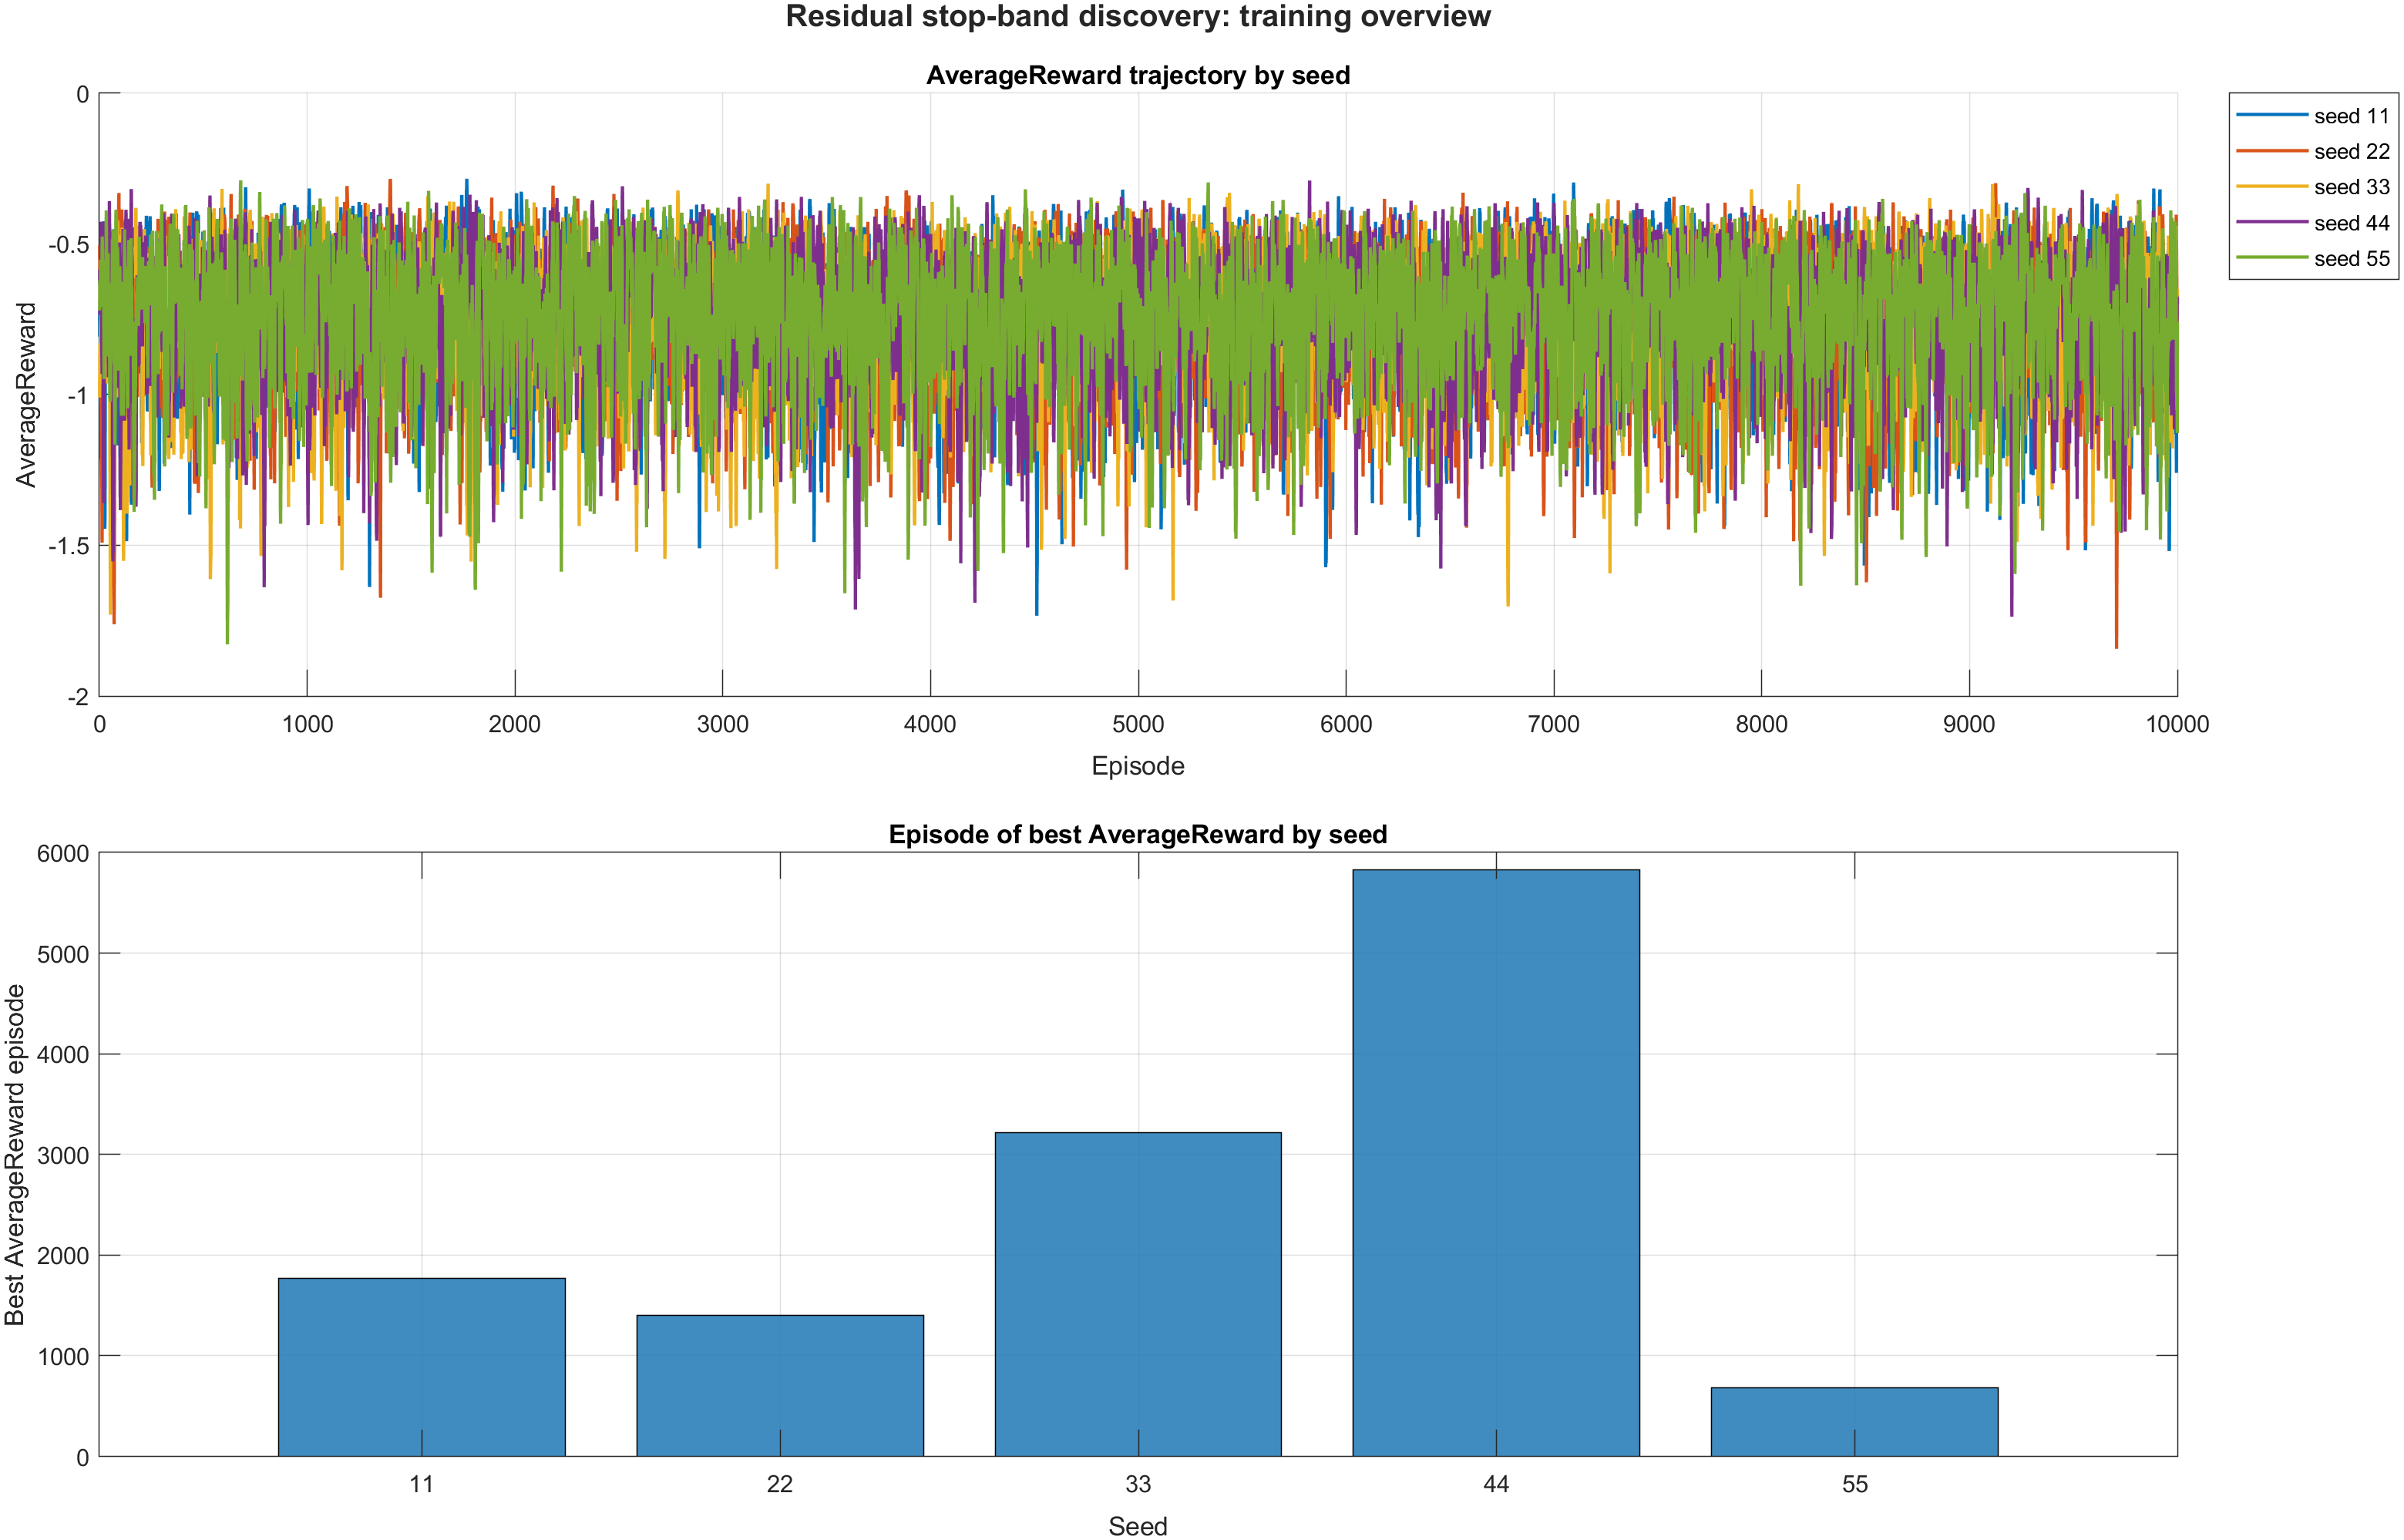
\includegraphics[width=\linewidth]{figures/residual_stopband_discovery_training_overview_20260405.png}
\caption{Vista general de entrenamiento por seed durante discovery. La dispersi\'on entre seeds confirma que discovery deb\'ia funcionar como fase de hip\'otesis, no de promoci\'on.}
\label{fig:discovery_training}
\end{figure}

\begin{figure}[H]
\centering
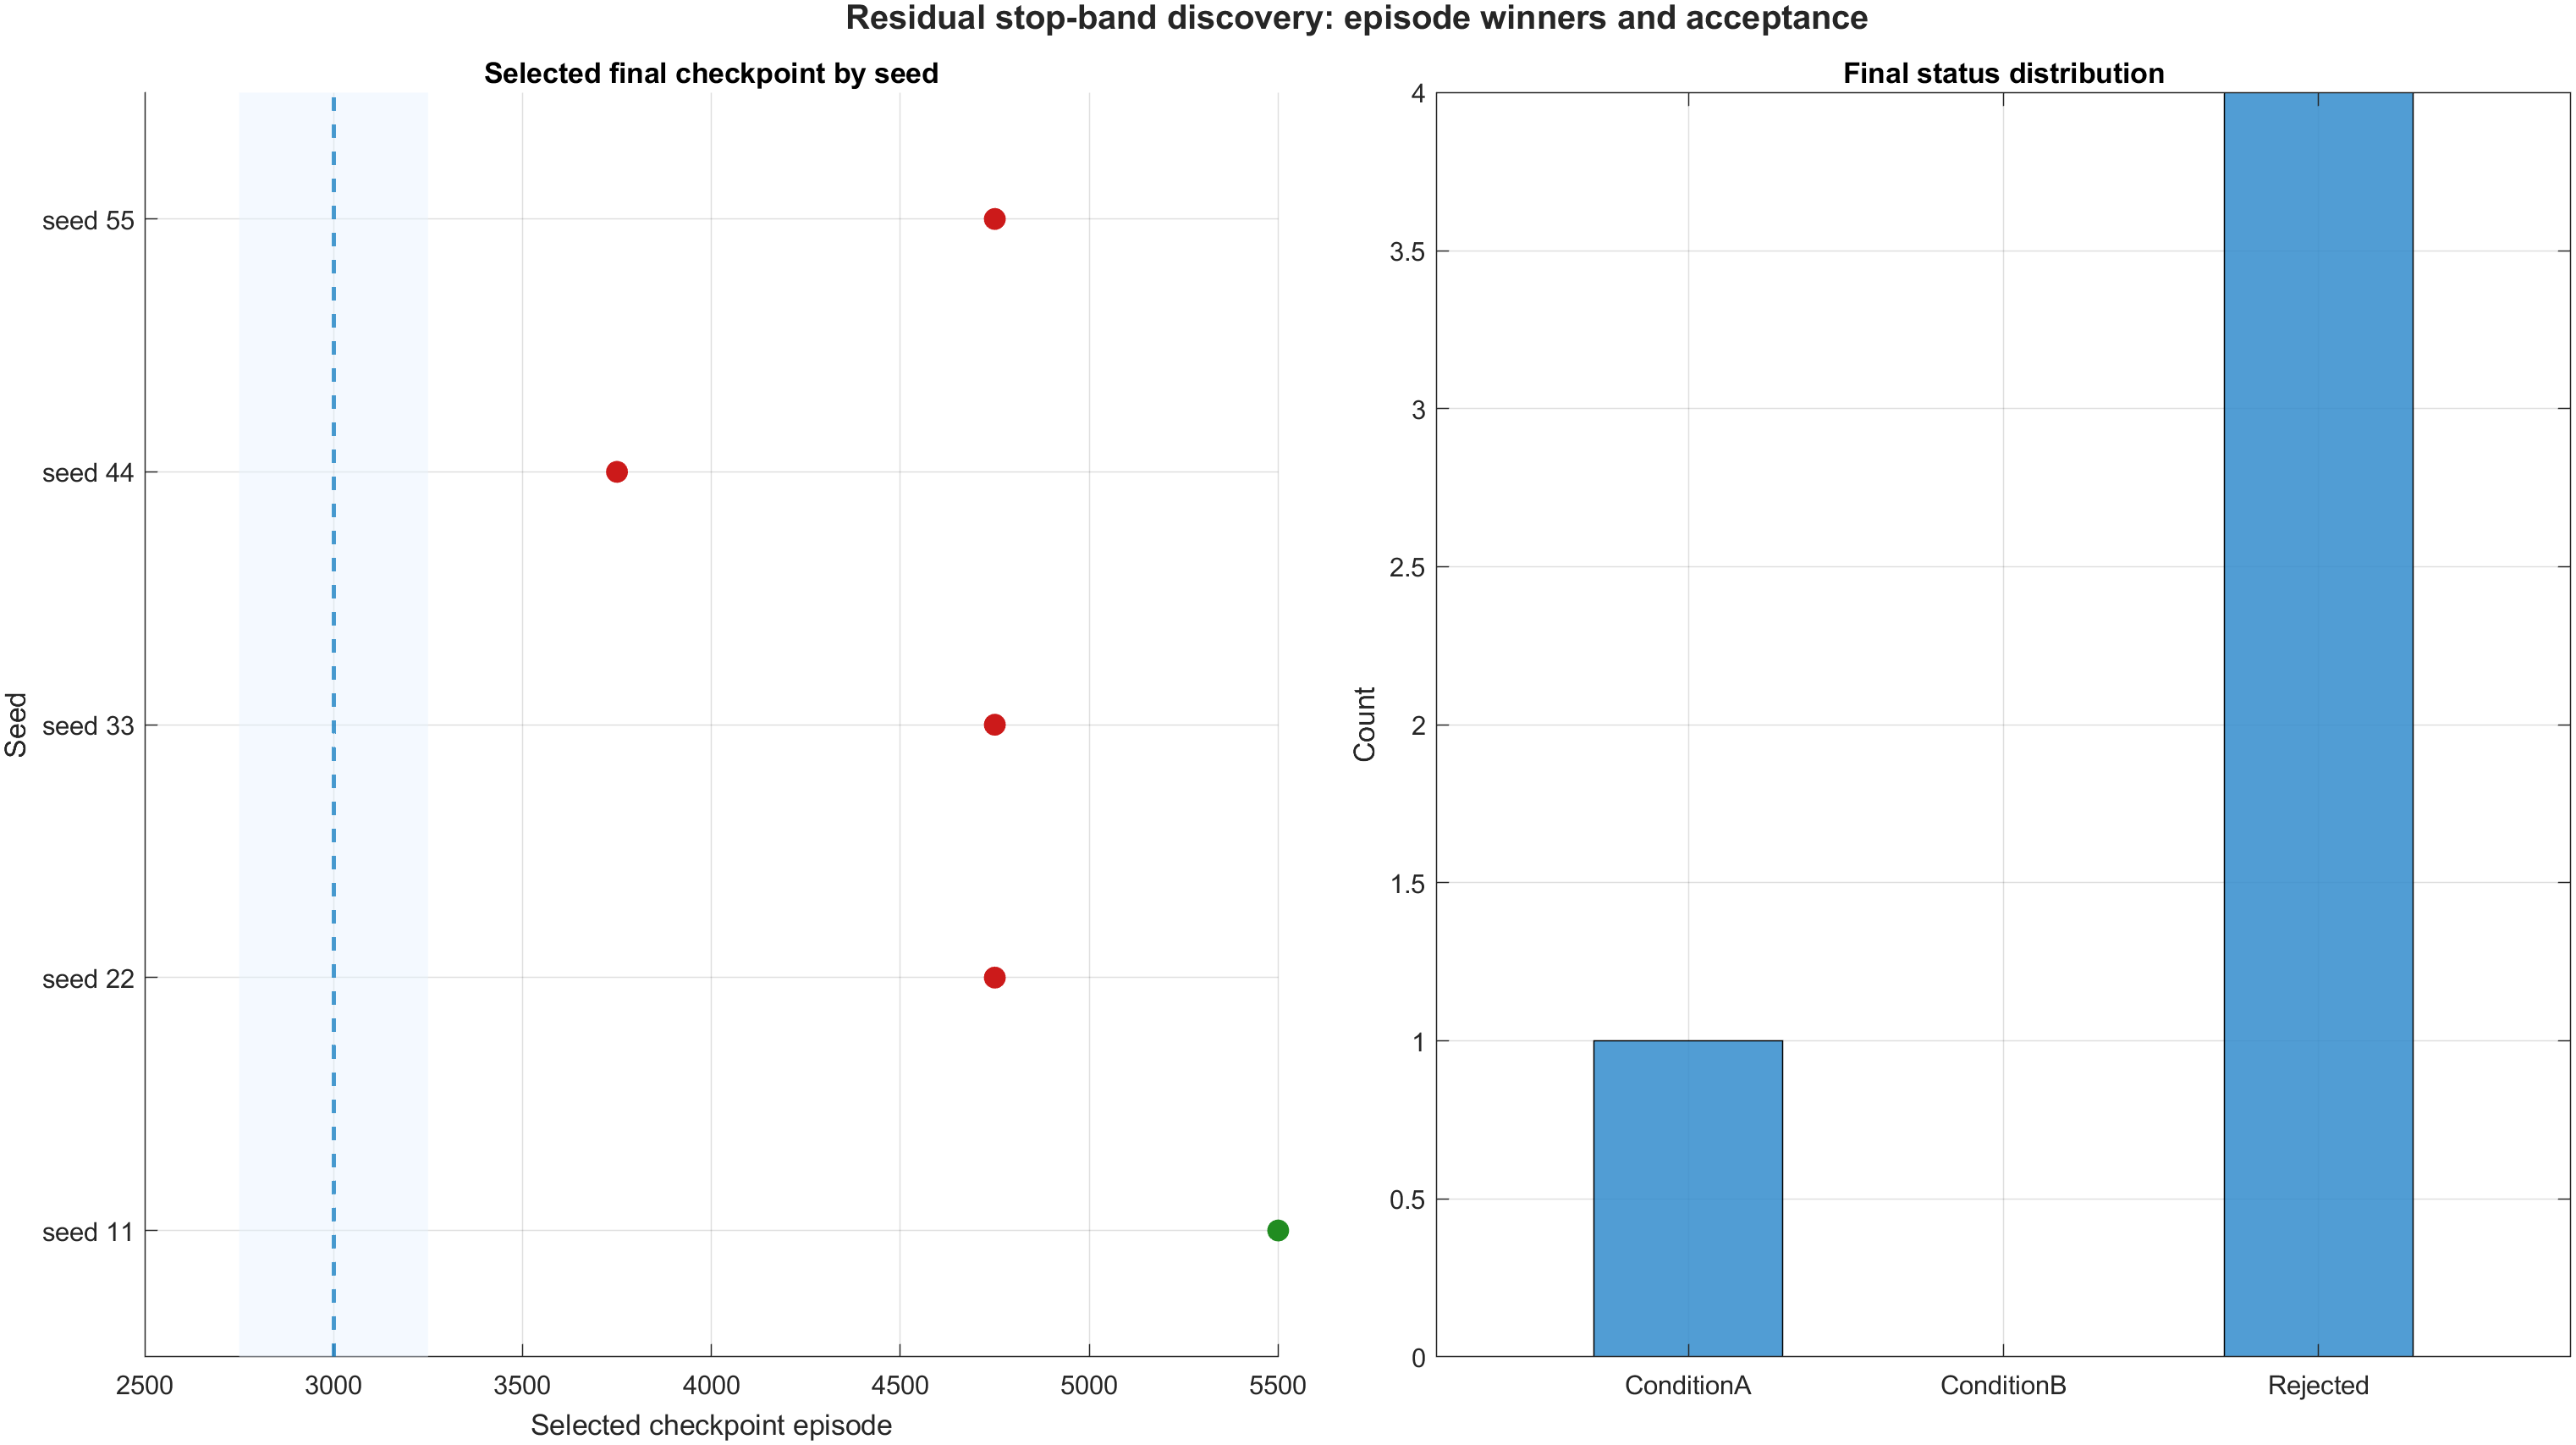
\includegraphics[width=\linewidth]{figures/residual_stopband_discovery_winner_episodes_20260405.png}
\caption{Episodios ganadores por seed y distribuci\'on final de estados en discovery. La banda propuesta nace de una evidencia a\'un escasa y por eso se mantiene conservadora.}
\label{fig:discovery_winners}
\end{figure}

\subsection*{Lectura}
Discovery \textbf{no estabiliz\'o la l\'inea por s\'i solo}. Solo una seed qued\'o aceptada y el promedio agregado termin\'o en \texttt{Rejected}. Esto es importante porque evita una lectura triunfalista equivocada: la fase inicial no ``demostr\'o'' una ventana, solo gener\'o una hip\'otesis de trabajo.

Sin embargo, discovery s\'i entreg\'o tres se\~nales \'utiles:
\begin{itemize}
\item mostr\'o que la mejora residual no estaba distribuida uniformemente a lo largo de toda la trayectoria;
\item mostr\'o que el mejor compromiso no aparec\'ia necesariamente al final de la corrida;
\item produjo una zona candidata concreta para someter a validaci\'on con seeds nuevas.
\end{itemize}

En t\'erminos de regla, discovery us\'o una mediana escasa y recortada. Eso es exactamente lo que deb\'ia pasar: con una sola seed aceptada, la fase no pod\'ia permitirse reaccionar como si ya hubiera evidencia reproducible.

\section*{Confirmation: validaci\'on de la banda}
\subsection*{Configuraci\'on}
\begin{table}[H]
\centering
\caption{Configuraci\'on de confirmation}
\begin{tabularx}{\linewidth}{lY}
\toprule
Elemento & Valor \\
\midrule
Base congelada & \texttt{Agent7250} \\
Seeds & \texttt{[66 77 88 99 111]} \\
stop-band de entrada & episodio \(3000\) desde discovery \\
Ventana de trabajo & \([2750, 3250]\) como referencia de entrada, con selecci\'on final re-evaluada por auditor\'ia y re-test \\
Episodios por seed & \(3500\) \\
Guardado & cada \(100\) episodios \\
Auditor\'ia & \(20\) simulaciones r\'apidas, \(50\) completas, \(\texttt{topK}=5\) \\
Selecci\'on final & checkpoint re-testeado; dentro de la ventana se prioriza el m\'as temprano aceptado \\
\bottomrule
\end{tabularx}
\end{table}

\subsection*{Resultado agregado}
\begin{table}[H]
\centering
\caption{Resumen agregado de confirmation}
\begin{tabularx}{\linewidth}{l c}
\toprule
M\'etrica & Valor \\
\midrule
Seeds aceptadas & \(3/5\) \\
ConditionA & \(2\) \\
ConditionB & \(1\) \\
Rejected & \(2\) \\
trackingMSE medio \(\pm\) std & \(0.042674 \pm 0.000490\) \\
trackingMAE medio \(\pm\) std & \(0.159880 \pm 0.000776\) \\
actionL2 medio \(\pm\) std & \(0.588257 \pm 0.037177\) \\
saturationFraction media \(\pm\) std & \(0.355790 \pm 0.080166\) \\
deltaActionL2 medio \(\pm\) std & \(0.368386 \pm 0.021190\) \\
Estado agregado vs benchmark & \texttt{ConditionA} \\
stop-band confirmada & episodio \(2000\) \\
Ventana confirmada & \([1750, 2250]\) \\
Promoci\'on de l\'inea activa & S\'i \\
\bottomrule
\end{tabularx}
\end{table}

\begin{figure}[H]
\centering
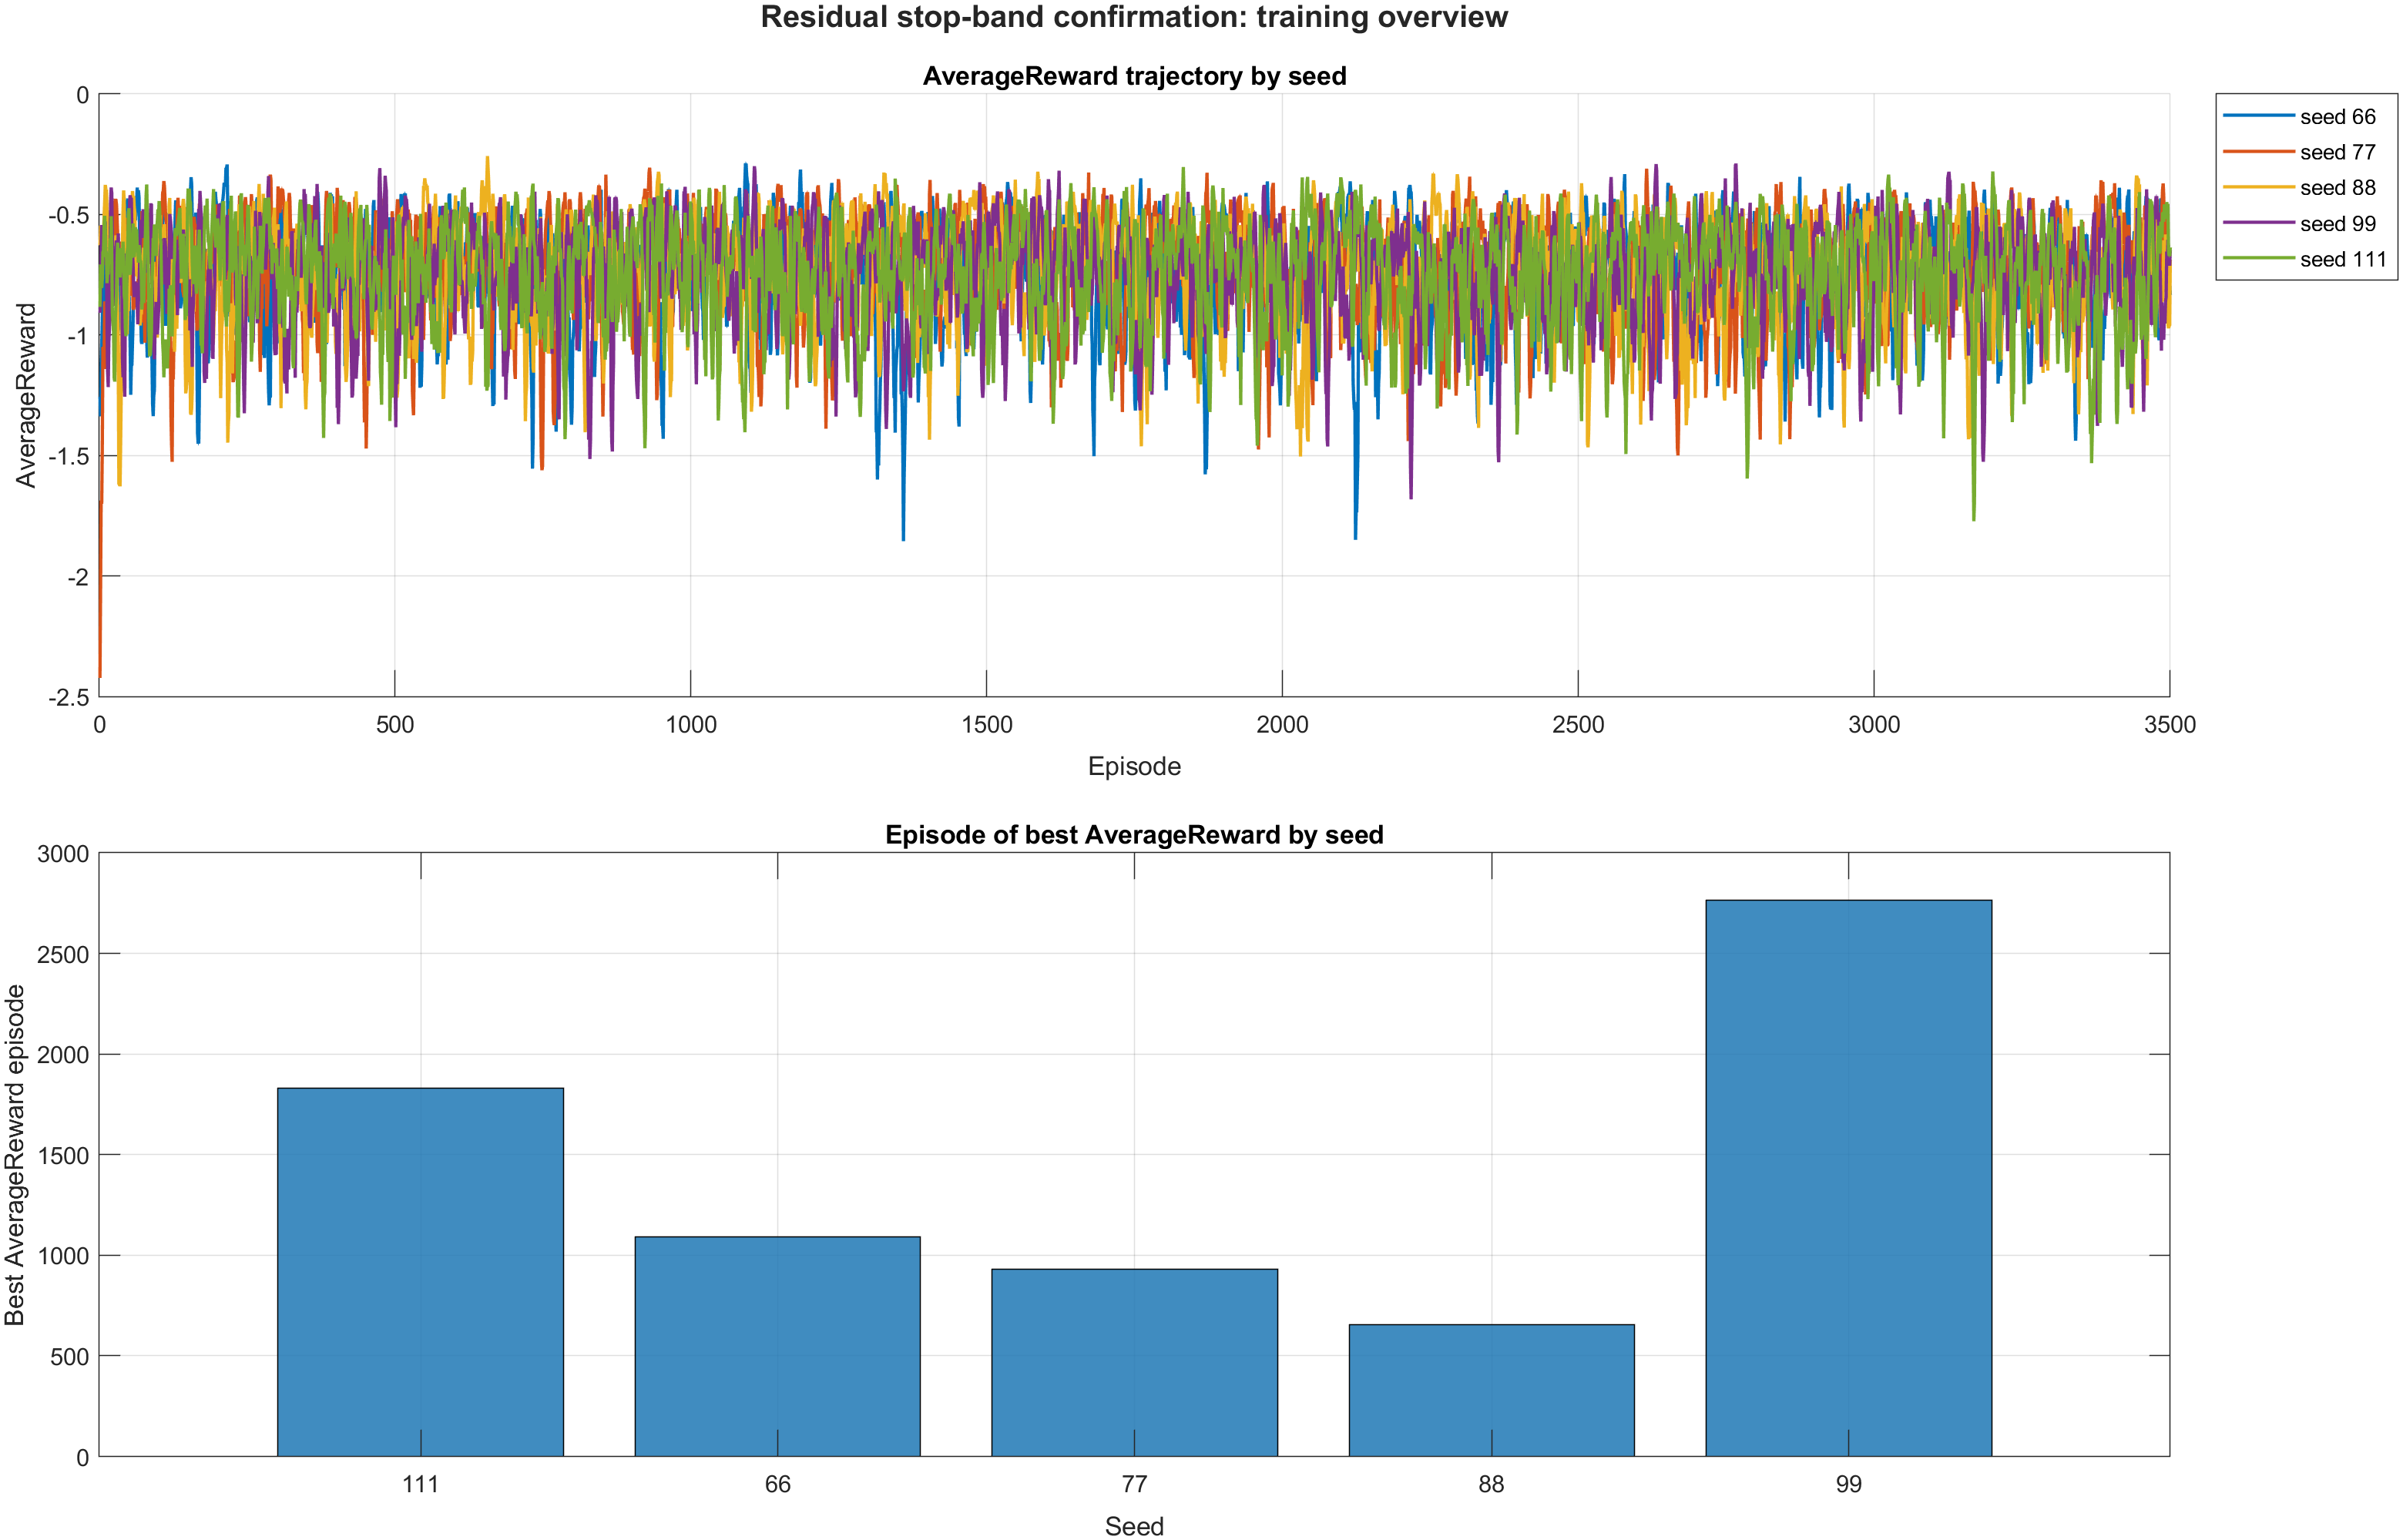
\includegraphics[width=\linewidth]{figures/residual_stopband_confirmation_training_overview_20260405.png}
\caption{Vista general de entrenamiento por seed durante confirmation. La concentraci\'on de buenos candidatos aparece m\'as temprano que la banda propuesta en discovery, lo cual refina la regla operativa.}
\label{fig:confirmation_training}
\end{figure}

\begin{figure}[H]
\centering
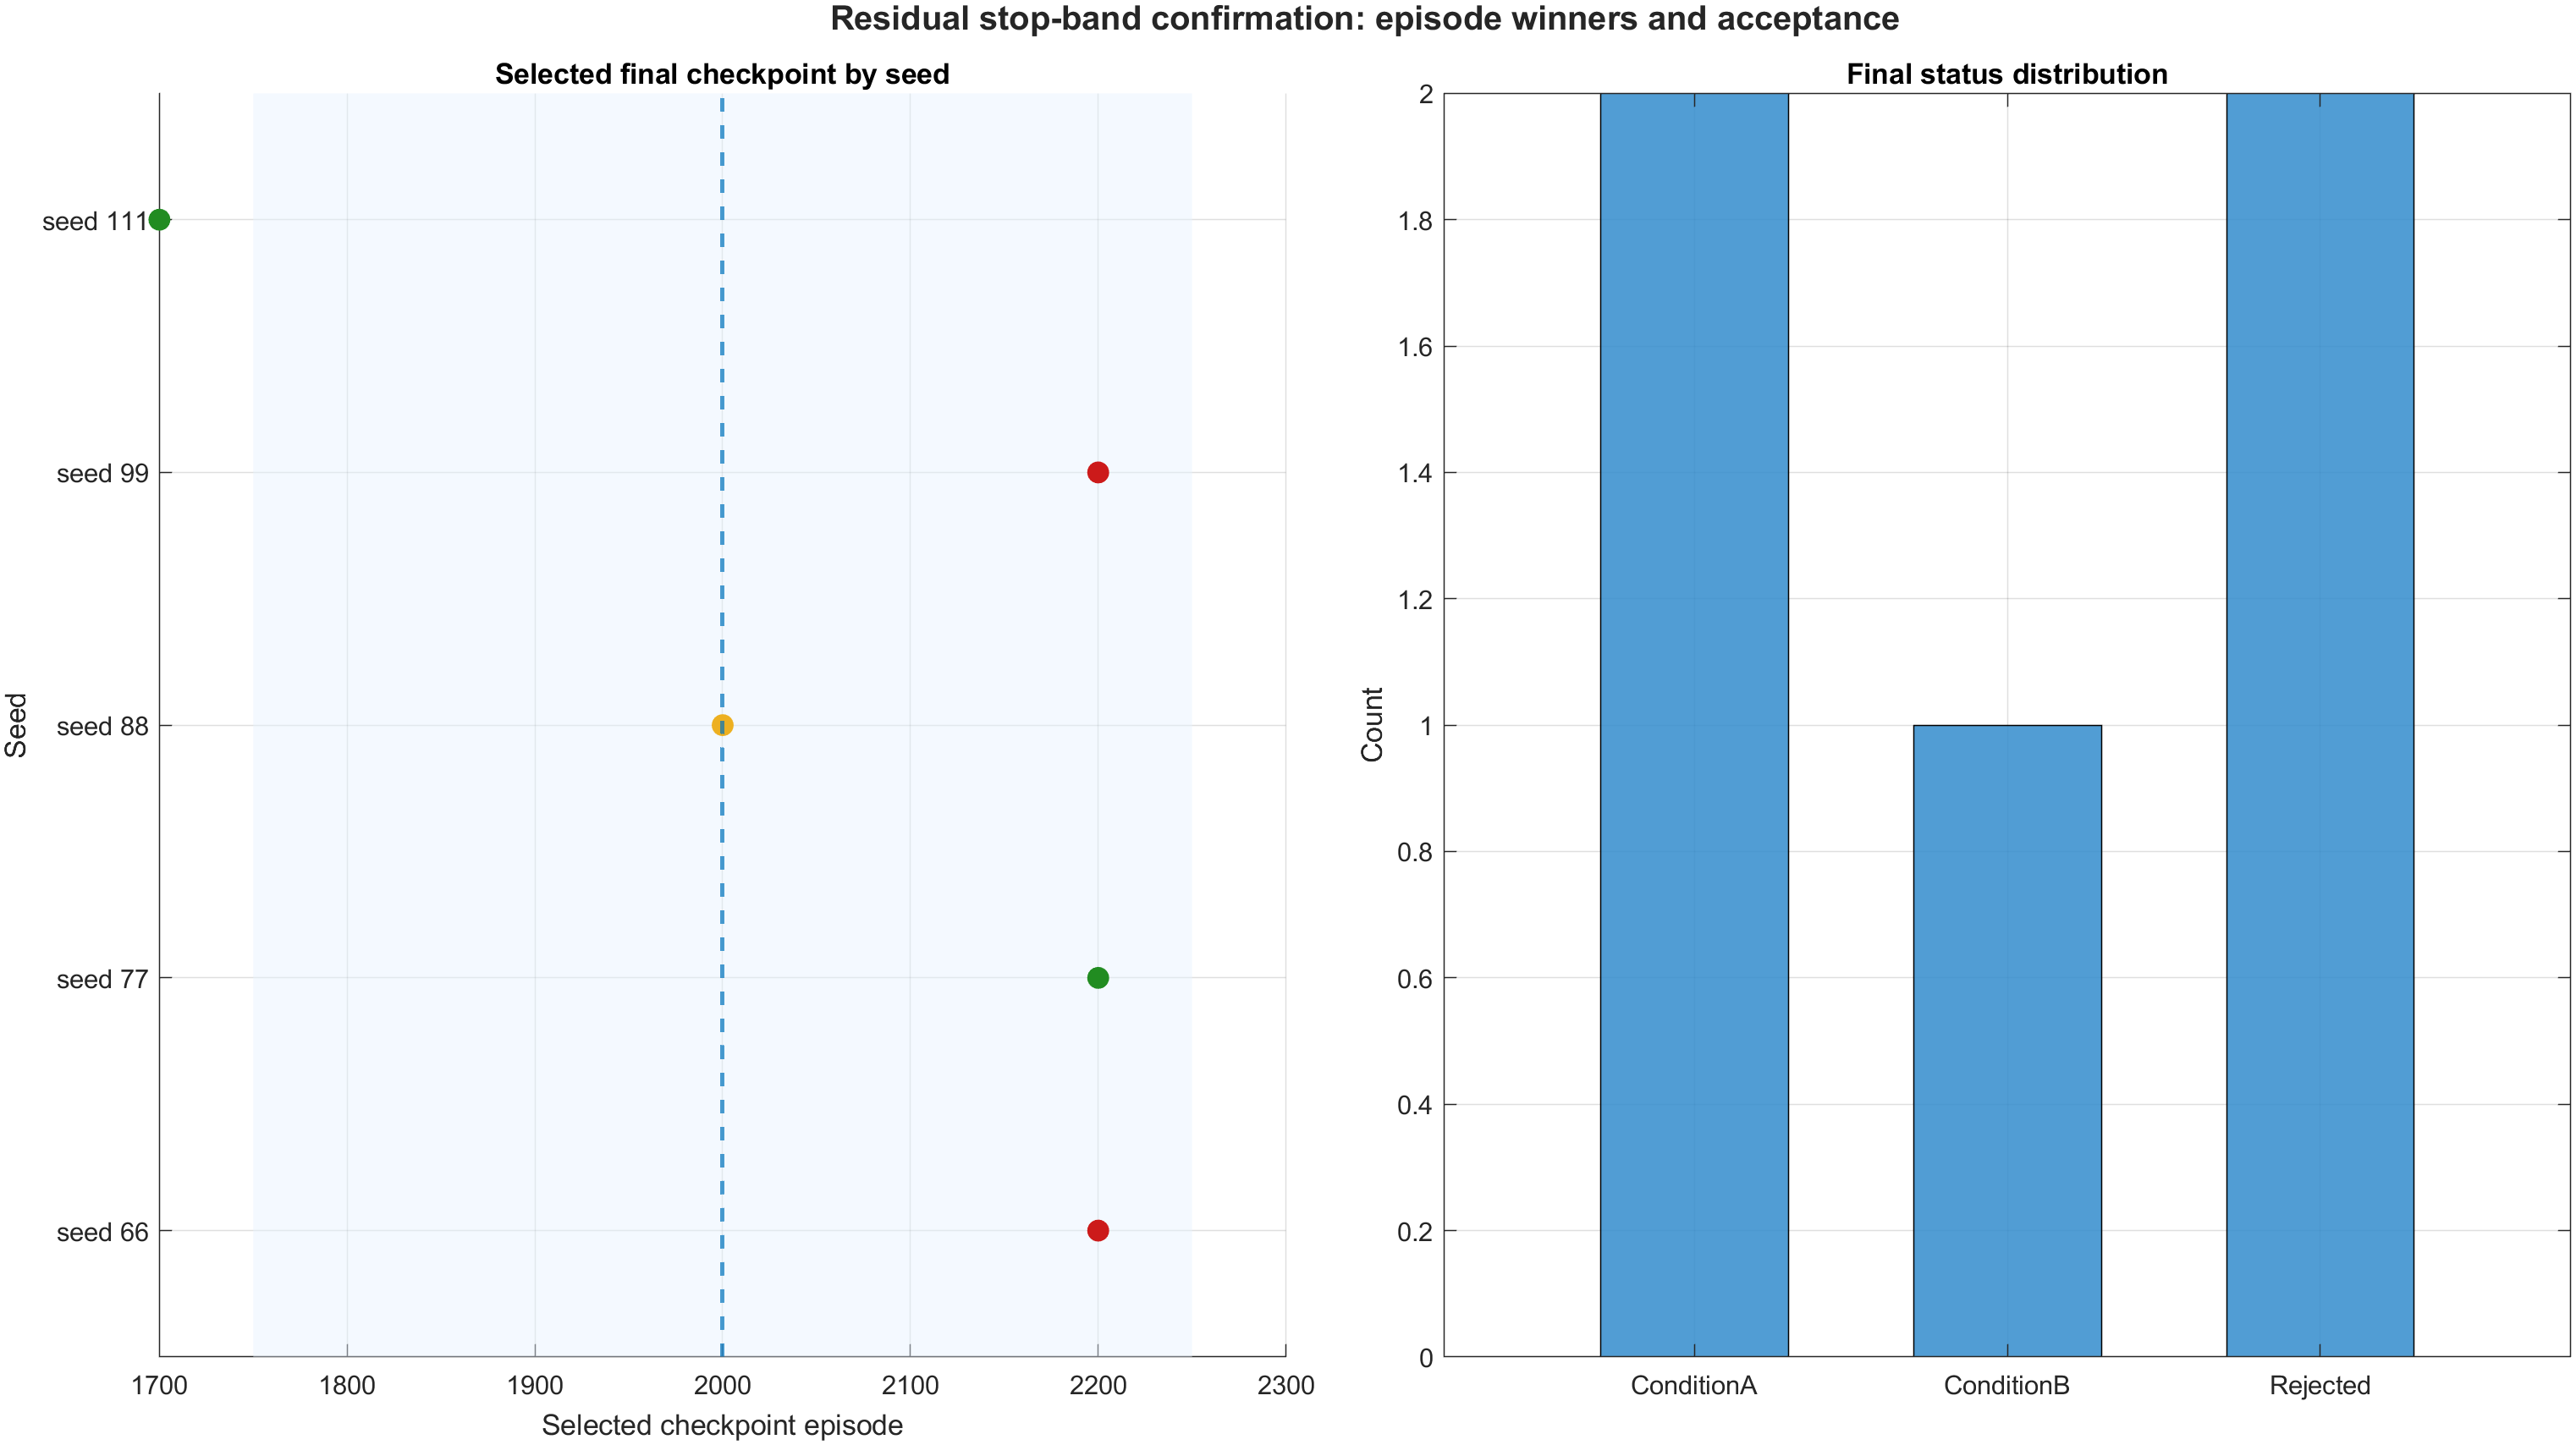
\includegraphics[width=\linewidth]{figures/residual_stopband_confirmation_winner_episodes_20260405.png}
\caption{Episodios ganadores por seed y distribuci\'on final de estados en confirmation. La mediana de las seeds aceptadas empuja la banda hacia \(2000\) episodios.}
\label{fig:confirmation_winners}
\end{figure}

\subsection*{Detalle por seed}
\begin{table}[H]
\centering
\caption{Checkpoint final seleccionado por seed en confirmation}
\scriptsize
\begin{tabularx}{\linewidth}{>{\raggedright\arraybackslash}p{1.0cm} c c c c c >{\raggedright\arraybackslash}p{1.5cm}}
\toprule
Seed & Episodio & trackingMSE & actionL2 & saturation & deltaActionL2 & Estado \\
\midrule
66 & 2200 & 0.043016 & 0.626795 & 0.439649 & 0.389861 & Rejected \\
77 & 2200 & 0.042057 & 0.553707 & 0.276106 & 0.346460 & ConditionA \\
88 & 2000 & 0.043291 & 0.545418 & 0.268202 & 0.353852 & ConditionB \\
99 & 2200 & 0.042400 & 0.619077 & 0.421728 & 0.392167 & Rejected \\
111 & 1700 & 0.042606 & 0.596287 & 0.373263 & 0.359592 & ConditionA \\
\bottomrule
\end{tabularx}
\end{table}

\subsection*{Lectura}
Aqu\'i apareci\'o la se\~nal fuerte de la fase. A diferencia de discovery:
\begin{itemize}
\item \(3/5\) seeds quedaron aceptadas;
\item la media agregada pas\'o a \texttt{ConditionA};
\item la banda confirmada se desplaz\'o hacia una zona \textbf{m\'as temprana}, entre \(1700\) y \(2200\) episodios;
\item la mediana de las seeds aceptadas produjo de forma natural una stop-band de \(2000\) episodios.
\end{itemize}

Esto significa que la hip\'otesis inicial se corrigi\'o a s\'i misma. Discovery propuso ``\emph{mira por aqu\'i}''; confirmation respondi\'o ``\emph{la zona buena s\'i existe, pero est\'a antes de lo que parec\'ia}''.

\section*{Comparaci\'on contra referencias activas}
\begin{figure}[H]
\centering
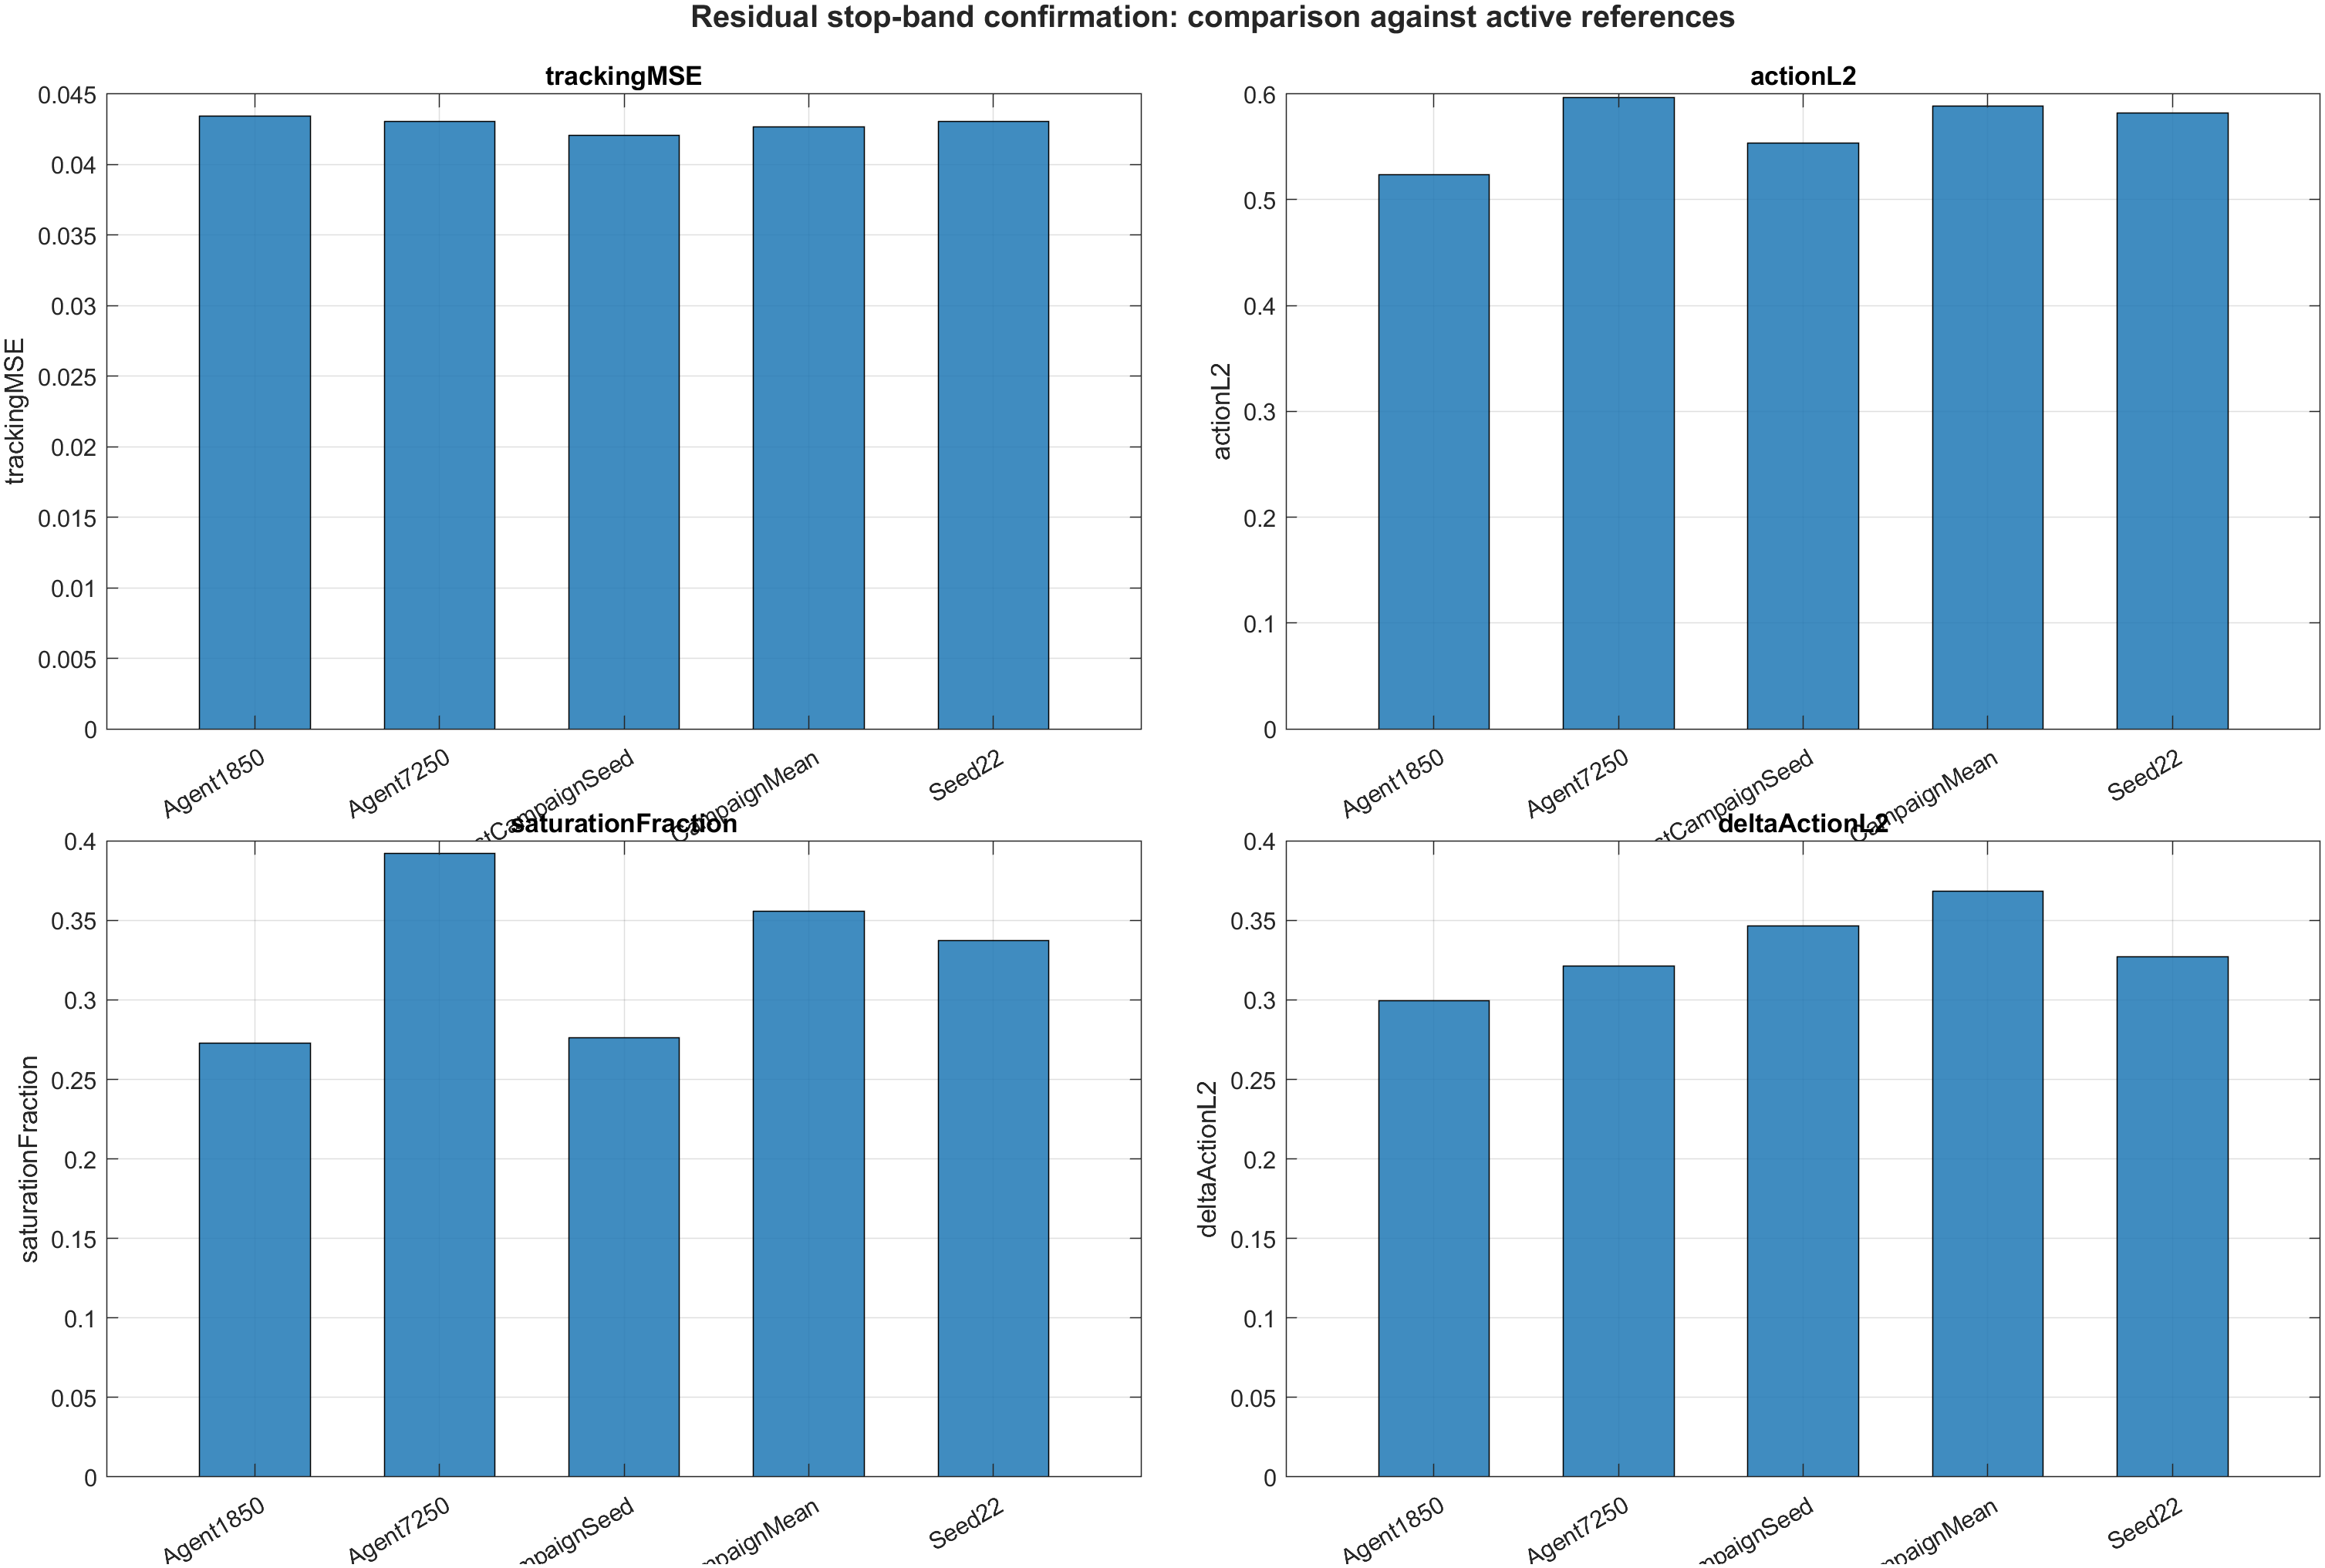
\includegraphics[width=\linewidth]{figures/residual_stopband_confirmation_comparison_20260405.png}
\caption{Comparaci\'on del resultado de confirmation contra \texttt{Agent7250}, \texttt{seed 22} y \texttt{Agent1850}.}
\label{fig:confirmation_comparison}
\end{figure}

\begin{table}[H]
\centering
\caption{Comparaci\'on final de referencias y campa\~na confirmada}
\scriptsize
\begin{tabularx}{\linewidth}{>{\raggedright\arraybackslash}p{2.2cm} c c c c c >{\raggedright\arraybackslash}p{1.6cm}}
\toprule
Candidato & trackingMSE & trackingMAE & actionL2 & saturation & deltaActionL2 & Estado \\
\midrule
Agent7250 & 0.043045 & 0.160336 & 0.596444 & 0.392086 & 0.321385 & Referencia \\
Seed22 & 0.043045 & 0.160786 & 0.582152 & 0.337475 & 0.327141 & ConditionA \\
Agent1850 & 0.043445 & 0.163542 & 0.523597 & 0.272637 & 0.299262 & ConditionB \\
MediaCampana & 0.042674 & 0.159880 & 0.588257 & 0.355790 & 0.368386 & ConditionA \\
MejorSeed & 0.042057 & 0.158791 & 0.553707 & 0.276106 & 0.346460 & ConditionA \\
\bottomrule
\end{tabularx}
\end{table}

\subsection*{Interpretaci\'on comparativa}
La fase confirmada deja una lectura bastante limpia:
\begin{itemize}
\item frente a \texttt{Agent7250}, la media confirmada mejora tracking y reduce tanto \texttt{actionL2} como \texttt{saturationFraction};
\item frente a \texttt{seed 22}, la campa\~na confirmada mejora tracking y mantiene una media aceptada, aunque \texttt{seed 22} sigue siendo una referencia reproducible muy fuerte;
\item frente a \texttt{Agent1850}, la stop-band confirmada no borra su valor hist\'orico: \texttt{Agent1850} sigue siendo un residual single-run sobresaliente en reducci\'on de esfuerzo y saturaci\'on, pero la nueva campa\~na gana como \textbf{l\'inea reproducible activa}.
\end{itemize}

Eso permite separar correctamente los roles:
\begin{itemize}
\item \texttt{Agent7250}: benchmark oficial estable;
\item \texttt{Agent1850}: mejor residual hist\'orico single-run;
\item campa\~na stop-band confirmada: nueva l\'inea residual activa para continuar.
\end{itemize}

\section*{Por qu\'e este resultado s\'i cambia el punto operativo}
La diferencia entre discovery y confirmation no es solo num\'erica; es metodol\'ogica. Discovery todav\'ia estaba en modo hip\'otesis. Confirmation, en cambio, cumpli\'o simult\'aneamente las condiciones que el propio proyecto se impuso para promover una l\'inea:
\begin{enumerate}
\item al menos \(3/5\) seeds en \texttt{ConditionA} o \texttt{ConditionB};
\item media agregada aceptada frente al benchmark;
\item \texttt{actionL2} media menor que \texttt{Agent7250};
\item \texttt{saturationFraction} media menor que \texttt{Agent7250}.
\end{enumerate}

Esto tiene una consecuencia pr\'actica clara. A partir de esta fase, el proyecto deja de privilegiar corridas largas ciegas y pasa a privilegiar:
\begin{itemize}
\item una base congelada fuerte;
\item residual learning controlado;
\item checkpoints densos;
\item auditor\'ia de trayectoria completa;
\item selecci\'on temprana dentro de una banda validada.
\end{itemize}

No es solo una preferencia de estilo experimental. Es una regla de operaci\'on mejor alineada con lo que este proyecto ya vio en sus corridas largas y con la forma en que la l\'inea residual realmente se comport\'o al extenderla demasiado.

\section*{Punto actual del proyecto}
El estado recomendado del proyecto queda fijado as\'i:
\begin{itemize}
\item \textbf{benchmark oficial}: \texttt{Agent7250};
\item \textbf{l\'inea residual activa}: \textbf{stop-band confirmada} alrededor del episodio \(2000\), con ventana \([1750,2250]\);
\item \textbf{mejor residual reproducible previo}: \texttt{seed 22}, ahora desplazado como referencia secundaria;
\item \textbf{mejor residual hist\'orico single-run}: \texttt{Agent1850}.
\end{itemize}

Operativamente, esto significa que ya no conviene seguir con corridas largas abiertas como estrategia principal. La recomendaci\'on para continuar es:
\begin{enumerate}
\item seguir usando \texttt{Agent7250} como base congelada;
\item entrenar residual con checkpoints densos;
\item auditar toda la trayectoria y no solo la cola;
\item priorizar checkpoints dentro de la ventana \([1750,2250]\);
\item elegir el checkpoint aceptado m\'as temprano dentro de esa banda;
\item usar esta ventana confirmada como plataforma para barridos finos o nuevas variantes.
\end{enumerate}

\section*{Veredicto final}
La fase stop-band residual fue exitosa.

No cambi\'o el benchmark oficial del proyecto, pero s\'i cambi\'o de forma clara la estrategia correcta para continuar. El valor principal de esta fase no es haber encontrado ``m\'as episodios'', sino haber demostrado que la parte \'util de la trayectoria residual aparece \textbf{antes} de la deriva tard\'ia y que esa zona puede validarse de forma reproducible con seeds nuevas.

La fase stop-band convierte una intuici\'on previa del proyecto en una regla experimental expl\'icita y defendible. La l\'inea vigente antes de la intervenci\'on ya mostraba que el residual era la v\'ia correcta; las corridas largas demostraron que empujar la trayectoria demasiado lejos no era la forma correcta de explotarlo; y la campa\~na discovery/confirmation mostr\'o que s\'i existe una banda temporal estable alrededor de \(2000\) episodios donde el residual ofrece el mejor compromiso operativo.

\bibliographystyle{plainnat}
\bibliography{references}

\end{document}
